\listfiles
\documentclass[a4paper,10pt]{report}

\author{Vladislav K. Valtchev} 
\title{IHPP: An Intraprocedural Hot Path Profiler}


\usepackage[utf8]{inputenc}
\usepackage[english]{babel}

\usepackage{hyperref}
\usepackage{xcolor,graphicx}
\usepackage{mdwlist}
\usepackage{fix-cm}
\usepackage{array}
\usepackage{tikz}
\usepackage{wrapfig}
\usepackage{listings}
\usepackage{cite}
\usepackage{cleveref}
\usepackage{makecell}
\usepackage{float}

%\usepackage{bold-extra}
%\usepackage[lighttt]{lmodern}
%\usepackage{pxfonts}
\usepackage[scaled=0.9]{couriers}

\addtolength{\textwidth}{1cm}
\addtolength{\textheight}{2cm}
\addtolength{\voffset}{-0.5cm}
\addtolength{\hoffset}{-0.5cm}

%%%%%%%%%%%%%%%%%%%%%%%%%%%%%%%%%%%%%%%%%%%%%%%%%%%%%%%%%%%%%%%

\usetikzlibrary{arrows,graphs,trees,fit,shapes,backgrounds,positioning}

\hypersetup{
    colorlinks,
    citecolor=black,
    filecolor=black,
    linkcolor=black,
    urlcolor=black
}

\lstset{
	basicstyle=\ttfamily\small, 
	%basewidth=0.5em,
	tabsize=4,
	keywordstyle=\bfseries,
	captionpos=b,
	framesep=10pt,
	numbersep=15pt
}


%in order to make the analytical index
%\usepackage{makeidx}
%\makeindex

\pagestyle{headings}

\begin{document}

\thispagestyle{empty}

\begin{figure}
\centering

\includegraphics[scale=0.6]{logo}
\end{figure}


\begin{center}


{\Large\textsc{Universit\`a degli studi di Roma}\\} 
{\huge\textsc{La Sapienza}\\[10pt]}
{\huge\textsc{Facolt\`a di Ingegneria}\\[40pt]} 

{\large Tesi di laurea in: \\}
{\LARGE\textsc{Ingegneria Informatica}\\[30pt]}

{\LARGE \textbf{IHPP}\\[10pt]\textit{An \textbf{I}ntraprocedural \textbf{H}ot \textbf{P}ath \textbf{P}rofiler}}\\[50pt]


\begin{tabular*}{0.9\textwidth}{@{\extracolsep{\fill}} @{} c @{} c @{} }
{\normalsize Docente relatore: } & {\normalsize Autore:}\\
{\large \textit{Prof. Camil Demetrescu} } & {\large \textit{Vladislav K. Valtchev}}\\
\end{tabular*}

\mbox{}\\[90pt]

{\large Anno accademico: 2011/2012\\}


\end{center}

%in order to print the analytical index
%\printindex

\pagebreak

%\thispagestyle{empty}
%
%\begin{center}
%
%\vspace*{4.5cm}
%
%\fontsize{70}{90}\selectfont \textbf{IHPP}\\
%\fontsize{20}{35}\selectfont
%\textit{An \textbf{I}ntraprocedural \textbf{H}ot \textbf{P}ath \textbf{P}rofiler}\\
%
%\vspace{11cm}
%
%\fontsize{14}{20}\selectfont
%\textbf{Vladislav K. Valtchev}
%
%\end{center}
%\pagebreak

\begin{abstract}
dwehkhjrkweh rlkewrhwe lkrhwek rhwel krhjweklrh welkrh wekrhwe krhwr
werwerwekr h jwekj rhwk jrhwk rhwl kjrh k kqhe qe wrkjehr r hk rhj
wlhrwelkjrfh sd hf kjh sdfkh jq ql lkqjhekqj q eqhkjeqkj kjahq 
erhjwe skafhd lkaerh welrk liwer  iwerh wit wielr qierhu lqr 
dwehkhjrkweh rlkewrhwe lkrhwek rhwel krhjweklrh welkrh wekrhwe krhwr
werwerwekr h jwekj rhwk jrhwk rhwl kjrh k kqhe qe wrkjehr r hk rhj
wlhrwelkjrfh sd hf kjh sdfkh jq ql lkqjhekqj q eqhkjeqkj kjahq 
erhjwe skafhd lkaerh welrk liwer  iwerh wit wielr qierhu lqr 
dwehkhjrkweh rlkewrhwe lkrhwek rhwel krhjweklrh welkrh wekrhwe krhwr
werwerwekr h jwekj rhwk jrhwk rhwl kjrh k kqhe qe wrkjehr r hk rhj
wlhrwelkjrfh sd hf kjh sdfkh jq ql lkqjhekqj q eqhkjeqkj kjahq 
erhjwe skafhd lkaerh welrk liwer  iwerh wit wielr qierhu lqr 
dwehkhjrkweh rlkewrhwe lkrhwek rhwel krhjweklrh welkrh wekrhwe krhwr
werwerwekr h jwekj rhwk jrhwk rhwl kjrh k kqhe qe wrkjehr r hk rhj

\end{abstract}


\tableofcontents

\chapter{Introduction}

In a world like today's one where computers are everywhere and where
\mbox{Internet} has more than 2.2 billion users, software has become more
important than ever. Today's operating systems have to handle much more
processes than in the past and every single process is often much more ``heavy''
than before due a great deal of reasons including (but not limited to): the
demand of users for much more complicated tasks (for example the multimedia
related ones), the intensive use of software layers by the programmers, the use
of high-level interpreted languages and many others. Thus, even if performance
of hardware is still growing following Moore's law and actual computers are
thousands times faster than before, they still to be ``slow'' sometimes and
software still needs to be analyzed and optimized. One way of analyzing
performance of programs is \textbf{profiling}: it consists substantially in
running the target program in a controlled environment and collecting data about
its behavior in order to discover possible bottlenecks in software. A basilar
introduction of program analysis and various profiling techniques can be found
in chapter 2.

\section{Actual profilers}

There are many profiler types today and a discrete number of profilers for
each category (as readers can see in the next chapter). But, \emph{most of them}
have two characteristics in common:

\begin{itemize*}

\item They focus only on procedures: data such counters and timers are collected
only on the procedure basis. This means that there is no way to understand what
happened \emph{inside} the procedures which caused, for example, a bottleneck.

\item Data has almost no \emph{calling context}, for example: it is possible to know that
a function \verb|a()| was called 10 times in a certain program, but it is not possible to know which were the \emph{callers} of \verb|a()|. Some profilers like \textbf{Valgrind} can
produce data with 2 levels of context: this means it is possible to know, for
example, that \verb|a()| was called 10 times, 3 of them by function
\verb|b()| and 7 of them by function \verb|c()|. This is better, but sometimes
it is not enough.

\end{itemize*}

Even if it is not too difficult to collect data with full context (infinite
levels) which is called ``building a CCT'' \emph{(calling context
tree)}, this often is practically useless because it grows too much specially due to
functions recursion~\cite{kccf}: the CCT is often too big to be physically stored and copied
simply and it is too big to be human-analyzable.
Thus, in the last years a few researches in theoretical computer science 
proposed different approaches for solving this problem and collecting \textbf{not fully context-sensitive} data. IHPP, the project described in this paper, uses one of these approaches called \textbf{$k$-CCF} (after explained).

\section{Motivations}

The aim of creation of IHPP was to make something that allows the study of
function calls with an arbitrary number of calling contexts but also to go
beyond the concept of procedure-only profiling: IHPP uses same ideas of
procedure-profiling to study the execution flow of basic blocks \emph{inside}
 functions. This sometimes can be really useful when there is a bottleneck in
the algorithm used for solving a problem: the programmer already knows which are
the \emph{slow functions} but he is still unaware of \emph{where exactly}
the problem is. Imagine functions with 3 loop levels and many conditional
statements: it is not trivial to understand where the problem is, neither to
solve it. But, even if a profiler \emph{will not} tell the programmer \emph{how}
to solve the problem, it will tell \emph{quickly} where is it, which is much
better than nothing because it can save several hours of programmer's work.

\section{Contributions}

In order to collect k-level context-sensitive data, IHPP uses some data
structures and algorithms that \emph{have not been} ideated by the author:

\begin{itemize*}
\item k-SF \emph{(k-Slab Forest)}
\item k-SF construction algorithm\footnote{This algorithm is used in the \textbf{traceObject()} function}
\item k-CCF \emph{(k-Calling Context Forest)}
\item Forest \emph{join} and $inv_k$ operations\footnote{These two operations should
be intended as \emph{theoretical} operations: in IHPP concrete algorithms have been
developed by the author}
\end{itemize*}

For these great and innovative data structures and algorithms, the author warmly
thanks \emph{Giorgio Ausiello}, \emph{Camil Demetrescu}, \emph{Irene Finocchi}
and \emph{Donatella Firmani}, professors at the \emph{Sapienza University of
Rome}\footnote{Officially, \textbf{Universit\`a degli studi di Roma ``La
Sapienza''}}.
Their work, called \emph{\mbox{k-Calling} \mbox{Context} \mbox{Profiling}}, has
been accepted for the \emph{27th \mbox{ACM} \mbox{SIGPLAN} Conference on
Object-Oriented Programming, Systems, Languages and Applications (OOPSLA 2012)}.

\section{Thesis structure}

\chapter{Program analysis}
The short introduction of before used the concept of \emph{profiling} without
too many explanations.
Instead, the goal of this chapter is to explain a \emph{little more} about
profiling contextualizing it in the more general concept of program analysis.
This kind of \emph{scientific background} has an encyclopedic form and
absolutely has no claim to be a good and an exhaustive coverage about the
subject since it is not the purpose of this paper.

Program analysis is the process of analyzing the behavior of computer
programs. Main applications of program analysis are 
\emph{program correctness checking} and \emph{program optimization}.
There are two main approaches in program analysis: static analysis and dynamic analysis.
The main difference between them is that in \emph{static} analysis nothing is
executed: the analysis is conducted only by observing the program source code or
the compiled program instructions. Instead, the \emph{dynamic} program analysis
is based on executing the program and observing what is it doing, even in real
time if possible.

\section{Static analysis}

Static analysis can be done either by hand or by using another program.
Information obtained by static analysis can be used in many ways, from
highlighting possible coding errors to application of formal methods that
mathematically prove some required properties of the algorithms used. It is
necessary to say, even if this is not the right context, that, as the work of
Alan Turing proved, there is no way to prove the absolute
correctness of an arbitrary program because of the \emph{halting
problem}~\cite{Turing01}.
By the way, there are many methods that give us estimated solutions with a
good level of reliability. We can mention four ways of doing static program
analysis:


\begin{description}
\item[Model checking] considers systems that have finite state or may be reduced to finite state by abstraction
\item[Data-flow analysis] is a lattice-based technique for gathering information about the possible set of values
\item[Abstract interpretation] models the effect that every statement has on the
state of an abstract machine (i.e., it 'executes' the software based on the
mathematical properties of each statement and declaration)
\item[Use of assertions] in program code as first suggested by Hoare
logic~\cite{Hoare01}
\end{description}

A more in deep explanation of these approaches goes too far away from the purpose of this paper.

\section{Dynamic analysis}

Dynamic program analysis is a form of analysis substantially based on the execution of the \emph{target program} in a sort of ``controlled environment''.
This definition is a quite generic because there many different ways of doing
this type of analysis as there are different objectives that who does the
analysis wants to achieve. For example, it can be done in order to trace memory
allocations (and discover memory leaks), to discover race conditions, memory
corruption, security vulnerabilities and also to do a \emph{performance
analysis}, which is often called \textbf{profiling}. It is usual to refer as \emph{profiling} when
the final goal of the work is to improve the program  \emph{performance} and
not, for example, to improve program \emph{correctness}: a memory analysis
is always a dynamic analysis but is not always a form of \emph{profiling}.

\subsection{The profiling}
The profiling is probably the most common form of dynamic program analysis and
its goal is, to analyze the performance of a program: the
\emph{performance} can be the amount of memory used, the frequency of certain
instructions, the frequency and/or the time consumption of some
\emph{procedures} / \emph{basic blocks} inside certain procedures. 
It is interesting here to focus the attention on the last kind of profilers; 
they can classified in two ways: according to the type of output and according to the method of data acquisition. Using the first classification rule, the following distinctions can be done:

\begin{description}
\item[Flat profilers] \hfill \\
These profilers count the number of function calls and/or average cpu time used
by each function without keeping trace of the calling context of the function.
\item[Call-graph profilers] \hfill \\
These profilers do the same things flat profilers do but also produce in output
the call-chains involved on the callee, which means that it is possible to know,
at the end of the execution of the target program, for every function, say it
$f()$, which functions were called by $f()$, which functions were
callers of $f()$ and how many times each function called each other. With this
information, it is possible to draw a
\emph{call-graph} like the one in figure~\ref{callgraph1}. But, this is
\emph{not} calling context profiling (which is what \textbf{IHPP} does) because,
for example, there is information such: $f()$ called $b()$ 8 times and $f()$ was called 20
times, 5 by $x()$ and 15 by $y()$ but there is \emph{not info} about how many times the
distinct calling sequence $x()\rightarrow f()\rightarrow b()$ occurred and how
many times the other calling sequence $y()\rightarrow f()\rightarrow b()$
occurred.

\begin{figure}

\begin{center}

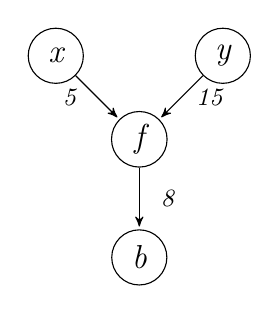
\begin{tikzpicture}
[->,>=stealth',shorten >=1pt,
node distance=1.5cm,
minimum size=7mm,
main node/.style={circle, draw, font=\itshape\large}]

  \node[main node] (1) {x};
  \node[main node] (3) [below right of = 1] {f};
  \node[main node] (2) [above right of = 3] {y};
  \node[main node] (4) [below of = 3] {b};

  \path[every node/.style={font=\itshape\small}]
    
    (1) edge node [left] {5} (3)
    (2) edge node [right] {15} (3)
    (3) edge node [right] {8} (4);
    
\end{tikzpicture}

\end{center}

\caption{A call graph}
\label{callgraph1}

\end{figure}



\end{description}

\begin{flushleft}
Instead, classifying profilers according to the method of data acquisition:
\end{flushleft}


\begin{description}
\item[Event-based profilers] \hfill \\
Some high-level languages and frameworks have they ad-hoc profilers based on
events. For example, \textbf{Java} has \textbf{JVMPI} \textit{(Java Virtual
Machine Profiling Interface)}, while in \textbf{.NET} it is possible to attach a
profiling agent as COM server to a .NET program using the \emph{Profiling APIs}.
These profilers are called \emph{event-based} because statements (of the
relative intermediate language) like function calls (or returns), object
creations (and many others \ldots) have \emph{traps} handled at low-level by the
relative virtual machine which generates \emph{events} and propagates these ones
to the high-level user event-handlers objects.

\item[Statistical profilers] \hfill \\
This kind of profilers work by \emph{sampling} at regular intervals the
\emph{instruction pointer} of target program through \emph{software interrupts}.
This approach, of course, produces numerically approximate data, but allows the
program to run at near full speed. Common profilers of that kind are \textbf{AMD
CodeAnalyst}, \textbf{Apple Shark}, \textbf{Intel VTune} and \textbf{Intel
Parallel Amplifier}.

\item[Instrumentation profilers] \hfill \\
This kind of profilers are used for \emph{native programs}\footnote{A native
program is a program written in a compiled language like \textbf{C},
\textbf{C++}, \textbf{Pascal}: the result of the building is an executable
containing architecture-specific instructions. Instead, non-native programs (aka
managed programs) don't contain binary instructions: they contain
intermediate-language (IL) instructions which only the relative virtual machine
(VM) understand. In order to the program to run, their VM runtime compile IL
instructions into machine specific instructions. \textbf{Java} and \textbf{.NET}
technologies use intermediate languages called relatively \textbf{Bytecode} and
\textbf{MSIL}.} and need to add binary instructions to the target program in
order to ``catch events'' like function calls. Instrumentation profilers can be
classified by the way they ``add instructions'' to the target program:

\begin{description}
\item[Manual]
This approach consists in modifying target program source code adding additional
statements in certain locations. For example, it is possible to add profiling
statements at the beginning of a set of procedures and before every their
\verb|return| statement: this method of collecting data allows building function
call-graphs, call context trees and much more; also, this method can be very
reliable but it requires a considerable amount of work.

\item[Automatic source level] This approach is very similar to the last one but
differs from it in the fact that profiling statements are added automatically by
a tool according to an instrumentation policy.

\item[Compiler assisted] Using a \emph{complier assisted} instrumentation means
that the source code remains intact and is the compiler the one who adds
profiling instructions at compile time. A practical example is the \verb|gcc| compiler when
used with \verb|-pg| option: it produces an executable with profiling
instructions but (in the specific case of \verb|gcc|) they are executed only when the
target program is executed in \emph{profiling mode} by the specific tool
\verb|gprof|.

\item[Binary translation]
This approach consist of adding instructions to an already compiled binary executable.

\item[Runtime instrumentation]
In this case, the additional instructions are added at runtime after program is
loaded in memory or really a little before they are going to be executed by the
cpu. In order to this to happen, another program which has \emph{full control}
of the target one is needed. This approach is used by tools like
\textbf{Valgrind} and \textbf{Intel Pin}\footnote{Pin's official page:
\url{http://www.pintool.org}} which is the tool used for the \textbf{IHPP}
project, so it will be explained in detail later.

\item[Runtime injection] This technique is based on the same idea of the last
one but it an a more \emph{lightweight} approach: substantially it consists of
modifying the target program \emph{text} adding unconditional branch
instructions to helper functions. The tool which does this work does not have the
\emph{full control} of the target program but only partial. An example of tool
which belongs to this category is \textbf{DynInst}.

\end{description} 

\item[Profiling through a hypervisor/simulator] \hfill \\
This type of profilers analyze the target program by executing it with no
changes in a kind of \emph{virtual machine} which can have also some ad-hoc
hardware support or it can work by literally emulating every single program
instruction. This approach is not unusual today. Two historical softwares
which adopted this approach were IBM SIMMON and IBM OLIVER.

\end{description}

\chapter{Algorithms and data structures in IHPP}
Since IHPP uses new and not yet published\footnote{The conference in which will be presented the work \emph{k-Calling Context
Profiling}~\cite{kccf} will be held in October 2012, as written here:
\mbox{\url{http://splashcon.org/2012/}}} data structures like $k$-SF and $k$-CCF, at least a basilar explanation of these ones is \emph{strictly} necessary in this paper. 
Note: in order to remove every possible ambiguity about these data structures, 
formal definitions used in this chapter are literally taken from the original work.

\begin{wrapfigure}[19]{l}{5.4cm}
\begin{center}

\scalebox{0.9}{
\begin{tabular}{r|l}
\textbf{operation} & \textbf{curr. context} \\
\hline
start & $\langle$$\rangle$ \\
call(r) & $\langle$r$\rangle$ \\
call(a) & $\langle$r,a$\rangle$ \\
call(b) & $\langle$r,a,b$\rangle$ \\
return & $\langle$r,a$\rangle$ \\
return & $\langle$r$\rangle$ \\
call(c) & $\langle$r,c$\rangle$ \\
call(a) & $\langle$r,c,a$\rangle$ \\
call(b) & $\langle$r,c,a,b$\rangle$ \\
return & $\langle$r,c,a$\rangle$ \\
call(b) & $\langle$r,c,a,b$\rangle$ \\
return & $\langle$r,c,a$\rangle$ \\
return & $\langle$r,c$\rangle$ \\
return & $\langle$r$\rangle$ \\
return & $\langle$$\rangle$ \\
%\hline

\end{tabular}
}

\caption{an execution trace}
\label{callex1}
\end{center}
\end{wrapfigure}
The figure~\ref{callex1} is an execution trace of a very simple imaginary program\footnote{This example, like some other ones in this chapter, was taken, for simplicity, from the article \emph{k-Calling Context Profiling}~\cite{kccf}.}; on its right part a very important information is shown: the current \emph{calling context}. 
As mentioned in chapter 1, \emph{vertex profiling} consists of counting the number of calls of a function; context-sensitive profiling instead, consists of counting the number of activations of a \emph{path}. In order to clearly explain this concept, some formal definitions are necessary.

\textbf{Definition 1}: \emph{$k$-calling context}~\cite{kccf}. 
Let $\pi = \langle r,...,v\rangle$ be a calling context of $v$. The k-calling context of $v$
in $\pi$ is the maximal suffix of $\pi$ of length at most $k+1$.

For example, the $2$-context of $(r,c,a,b)$ is $\langle c,a,b\rangle$ and its $0$-context is $\langle b\rangle$.

\textbf{Definition 2}: \emph{Path activation}~\cite{kccf}. 
A path $\pi$ of length $q$ in the call graph of the program is activated by 
a \texttt{call(}$v$\texttt{)}
operation if $\pi$ is the $q$-context of $v$ resulting from the \texttt{call} operation.

\textbf{Definition 3}: \emph{$k$-calling context profiling}~\cite{kccf}. Given a trace
of \texttt{call} and \texttt{return} operations, the $k$-(calling) context
profiling problem consists of computing, for each activated path $\pi$ of length $q\le k$, the number $c(\pi)$ of times $\pi$ is activated.

The figure~\ref{kctx1} (below) shows, as a clarifying example, all $k$-contexts for $k=0,1,2,3$ of the execution trace illustrated by figure~\ref{callex1}:

\begin{figure}[h]
\begin{center}
\begin{tabular}{c|c|c}
$k$ value & \textbf{$\pi$} \emph{(k-context)} & $c(\pi)$ \emph{(activation counter)}\\
\hline
0 & $\langle$r$\rangle$* & 1\\
0 & $\langle$a$\rangle$ & 2\\
0 & $\langle$b$\rangle$ & 3\\
0 & $\langle$c$\rangle$ & 2\\
\hline
1 & $\langle$r,a$\rangle$* & 1\\
1 & $\langle$a,b$\rangle$ & 3\\
1 & $\langle$a,c$\rangle$ & 1\\
1 & $\langle$r,c$\rangle$* & 1\\
1 & $\langle$c,a$\rangle$ & 1\\
\hline
2 & $\langle$r,a,b$\rangle$* & 1\\
2 & $\langle$r,a,c$\rangle$* & 1\\
2 & $\langle$r,c,a$\rangle$* & 1\\
2 & $\langle$c,a,b$\rangle$ & 2\\
\hline
3 & $\langle$r,c,a,b$\rangle$* & 2\\

\end{tabular}
\end{center}
\caption{$k$-contexts for various values of $k$.
Note: contexts marketed with (*) are \emph{full} calling contexts.}
\label{kctx1}
\end{figure}

As it is possible to see, for various values of the $k$ parameter there are more or less $k$-contexts with different values of $c(\pi)$: for $k=0$ $c(\pi)$ is, simply, the number of times each function is called; for $k=2$ instead, $c(\pi)$ is number of times an unique 3-elements-path like $\langle$r,a,b$\rangle$ is activated. This example is too simple to show that but, in general, as $k$ grows, more context information is added but counter values decrease and, for relatively big values of $k$, information made become too specific for any sort analysis so, it is a profiler's user task to choose the \emph{right} $k$-value.

At this point, the problem is how to get (in terms of algorithms and data
structures) all $k$-contexts of a program run for a given value of $k$: a solution is to extract the $k$-contexts from a CCT (\emph{Calling Context Tree}) which is build
``observing'' the execution trace of the target program.

\section{The Calling Context Tree}

The CCT is the simplest data structure for handling full context-sensitive information: 
it consists of a tree which has as root-node the \emph{enter point} of the target program.
Every procedure called is represented in the tree by a children-node of its callee. 
The CCT of the execution trace considered until now is shown in figure~\ref{cct1}.
It is self-evident that the CCT contains all $k$-contexts for all values of $k$ even if 
it can be not obvious how a CCT is build or how $k$-calling contexts can be extracted from it.\\
An algorithm for building a CCT is the one in \cref{cct_alg}.


\begin{figure}[H]

\begin{center}
\scalebox{0.9}{
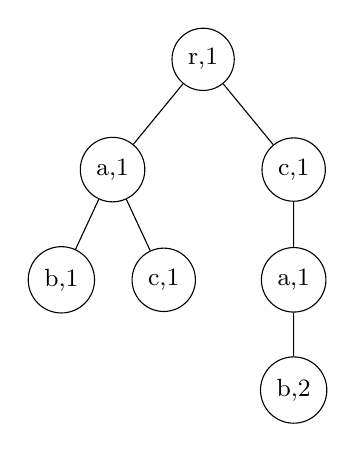
\begin{tikzpicture}[level distance=1.4cm,
  level 1/.style={sibling distance=2.3cm},
  level 2/.style={sibling distance=1.3cm},
  main node/.style={circle,draw,font=\small}]

\node[main node] {r,1}
	child { node[main node] {a,1}
		child { node[main node] {b,1} }
		child { node[main node] {c,1} }
	}
	child { node[main node] {c,1} 
		child { node[main node] {a,1}
			child { node[main node] {b,2} }
		}
	};


\end{tikzpicture}
}
\end{center}

\caption{The CCT of figure~\ref{callex1}. Nodes are labeled in this way: routine name, counter.}
\label{cct1}

\end{figure}

\newpage

\begin{lstlisting}[language=java, label={cct_alg}, caption={An algorithm for building a CCT}, morekeywords={function,then,endif},frame=leftline,framesep=10pt]
node treeRoot=null,currentNode=null

function func_call_event_handler(funcType func):

	if (currentNode == null) then 	
		currentNode = new node(func,1) 
		treeRoot=currentNode
		return
	endif

	node temp = currentNode.findNodeByFuncInChildren(func)

	if (temp == null) then
		temp = new node(func,1)
		currentNode.addChildren(temp)
	else
		temp.incrementCounter()
	endif

	currentNode=temp

function func_ret_event_handler():
	currentNode=currentNode.getParent()

\end{lstlisting}

The above code should be self-explaining.
The algorithm for extracting $k$-contexts from a CCT is a little more articulated 
and its pseudo-code will not be shown here but the idea is: given a CCT and a node $n$ of it, it is possible to get the $k$-context of $n$ taking the first (or at most) $k$ nodes from the path which joins $n$ with the root node; doing this for every node and summing counters of all distinct paths is enough for collecting all $k$-contexts of a CCT.

\section{The $k$-Calling Context Forest}

As told in \emph{k-Calling Context Profiling}~\cite{kccf}, building (and handling) a CCT for a relatively long running program is impractical and often useless.
A much better data structure for handling $k$-contexts is \emph{$k$-CCF}: 
the idea on which it is based is to have a \emph{forest} formed by 
a tree (of at most $k$ levels) \emph{for each} function. 

\begin{figure}[h]

\begin{center}
\scalebox{0.8}{
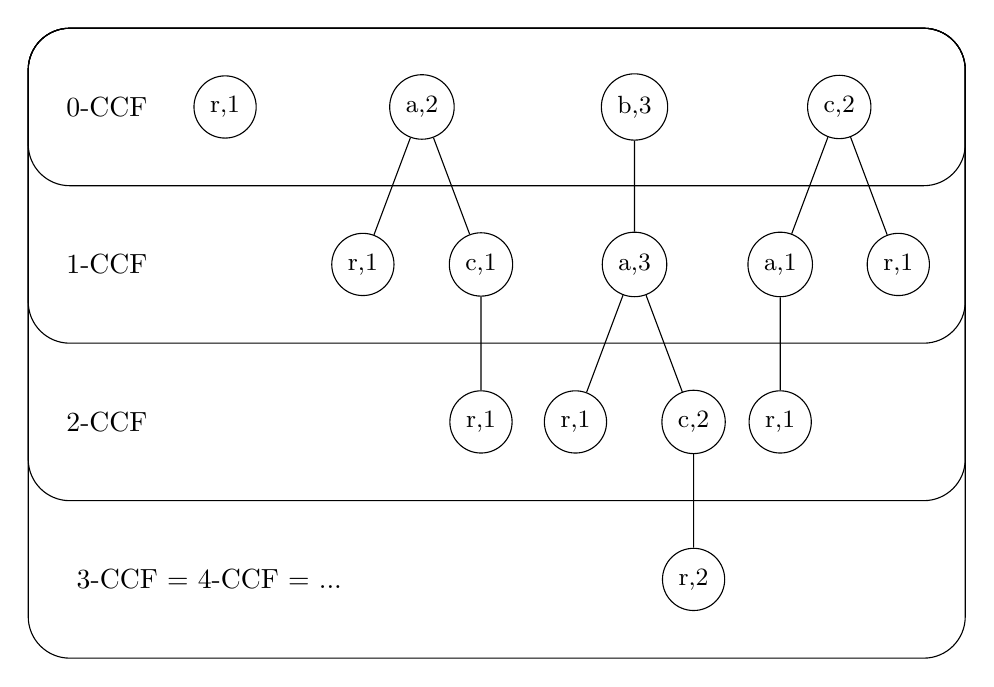
\begin{tikzpicture}[level distance=2.0cm,
  level 1/.style={sibling distance=1.5cm},
  level 2/.style={sibling distance=1.5cm},
  main node/.style={circle,draw,font=\small}]
  

  \node[main node] at (0, 0) {r,1};

  \node[main node] at (2.5, 0) {a,2} 
    child {
	   node[main node] {r,1}
    }
	child {
		node[main node] {c,1}
		child { node[main node]{r,1} }
	};


  \node[main node] at (5.2, 0) {b,3}
  child {
		node[main node] {a,3}
		child { 
			node[main node] {r,1}
		}
		child {
			node[main node] {c,2}
			child { node[main node] {r,2} }
		}
  };

  \node[main node] at (7.8, 0) {c,2}
  child {
		node[main node] {a,1}
		child { node[main node]{r,1} }
  }
  child { node[main node] {r,1} };

  \draw [rounded corners=15pt] (-2.5,-1) rectangle (9.4,1);
  \draw [rounded corners=15pt] (-2.5,-3) rectangle (9.4,1);
  \draw [rounded corners=15pt] (-2.5,-5) rectangle (9.4,1);
  \draw [rounded corners=15pt] (-2.5,-7) rectangle (9.4,1);

  \node at (-1.5,0) {$0$-CCF};
  \node at (-1.5,-2) {$1$-CCF};
  \node at (-1.5,-4) {$2$-CCF};
  \node at (-0.2,-6) {$3$-CCF = $4$-CCF = ...};

\end{tikzpicture}
}
\end{center}

\caption{$k$-CCF relative to CCT in fig.~\ref{cct1} for various values of $k$.}
\label{kccf1}

\end{figure}

The interpretation of fig.~\ref{kccf1} is simple: for $k=0$ there is no context
information and only one node per function is present; its counter shows the number of times that function has been called during the program execution. For $k=1$, every function has as children its callers, for example, $a()$ has been called $2$ times: 1 by $r()$ and 1 by $c()$. This way of proceeding can be extended for greater values of $k$ with the remark that 
there is always a maximum $k$-value which produces a full context-sensitive information 
(in this example, that value of $k$ is $3$): greater values of $k$ have no effect on the output. Apart of these considerations, $k$-CCF have not been formally defined yet because its definition uses an operation called \emph{tree join}.

\subsection{The join operation}

\textbf{Definition 4} \emph{Tree join}~\cite{kccf}. 
The join of two labeled trees $T_1$ and $T_2$, denoted as 
\texttt{\textbf{join(}}$T_1$\texttt{\textbf{,}}$T_2$\texttt{\textbf{)}}, 
is the minimal labeled forest $F$ such that $F$ contains a root-label path $\pi$ if and 
only if $T_1$ or $T_2$ contain $\pi$.

Note: if $T_1$ and $T_2$ have different root labels, 
formally if $l(r_1)\ne l(r_2)$, then $F$ will be simply a forest with two trees: $T_1$ and $T_2$. In order to deals with weighted trees, the join operation just defined have to be extended in this way: 
\newpage
\textbf{Definition 4*} \emph{Weighted tree join}~\cite{kccf}.
Let: 

\renewcommand{\labelitemi}{$-$}

\begin{itemize*}
\item $T_1$ and $T_2$ be two trees
\item $V_1$ and $V_2$ be all nodes of $T_1$ and $T_2$
\item $c(v)$ be a counter associated with each node $v$ in $V_1$ and $V_2$
\item $F$ be the weighted tree join of $T_1$ and $T_2$
\item $z$ be a node of $F$
\item $\pi_z$ be the unique root-path that leads to $z$ in $F$
\end{itemize*}
\renewcommand{\labelitemi}{$\bullet$}
$c(z)$ is defined as sum of all counters $c(v)$ of nodes $v$ in $V_1 \cup V_2$ such
that the root-path $\pi_z$ that leads to $v$ in $T_1$ or $T_2$ has the same sequence of 
labels as $\pi_z$.

\begin{figure}[h]

\begin{center}
\scalebox{0.9}{

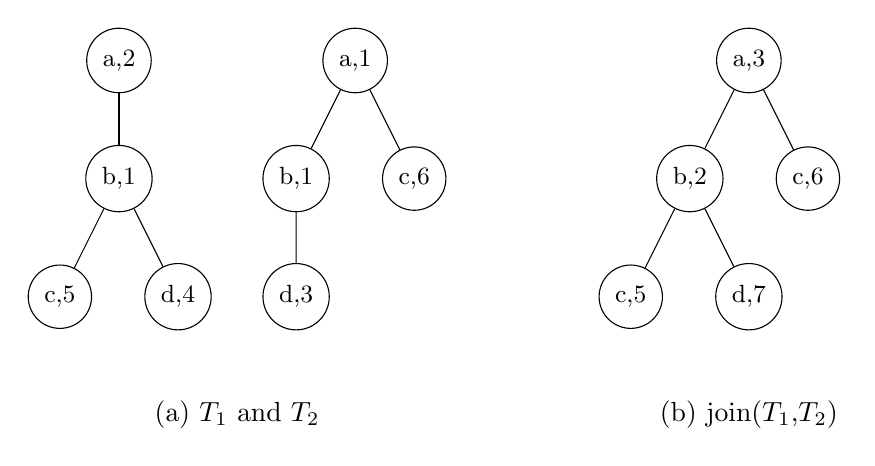
\begin{tikzpicture}[level distance=1.5cm,
  level 1/.style={sibling distance=1.5cm},
  level 2/.style={sibling distance=1.5cm},
  main node/.style={circle,draw,font=\small}]
  
  \node[main node] at (0,0) {a,2}
  child { 
		node[main node] {b,1}
		child {node[main node] {c,5}}
		child {node[main node] {d,4}}
  };

  \node[main node] at (3, 0) {a,1}
  child {
		node[main node] {b,1}
		child {node[main node] {d,3}}
  }
  child {
		node[main node] {c,6}
  };

  \node[main node] at (8, 0) {a,3}
  child {
		node[main node] {b,2}
		child {node[main node] {c,5}}
		child {node[main node] {d,7}}
  }
  child {node[main node] {c,6}};

  \node at (1.5, -4.5) { (a) $T_1$ and $T_2$ };
  \node at (8, -4.5) { (b) join($T_1$,$T_2$) };

\end{tikzpicture}
}
\end{center}

\caption{An example of the tree join operation}
\label{join1}
\end{figure}

Figure~\ref{join1} shows an example that should clarify the above definition:
$T_1$ and $T_2$ trees have a common root-node label, $a$, so they can be merged and 
both counters of $a$ can be summed; also, in both trees is present a path $\langle a,b\rangle$ so the counter of node $a\rightarrow b$ in the resulting tree 
is the sum of the counters of that path in trees $T_1$ and $T_2$; 
the same logic can be used for node $a\rightarrow b\rightarrow d$. 
Instead, paths $\langle a, b, c\rangle$ and $\langle a, c\rangle$ are not common 
in both trees so they exist in the merged tree, but no counters are summed.
The join operation can be extended for working with more than two trees.
let ($T_1$, ..., $T_h$), with $h > 2$, be a set of trees, then:
if all them have distinct root labels, the output forest $F$ will be the same
set of trees, otherwise, if for example $T_1$ and $T_2$ have the same root label,
the following expression could be written:
\begin{center}
\texttt{join($T_1$, \dots, $T_h$) $=$ join(join($T_1$,$T_2$),$T_3$, \ldots, $T_h$)}
\end{center}

\subsection{The formal definition of $k$-CCF}

At this point, $k$-CCF can be formally defined using its original definition.\\

\textbf{Definition 5} \emph{k-Calling Context Forest}~\cite{kccf}. The $k$-calling context
forest of the execution of a program is a labeled forest defined as 
\texttt{join}($\pi_1^R$, \ldots, $\pi_s^R$), where ($\pi_1$, \ldots, $\pi_s$) is the set of
all distinct paths of length a most k+1 activated by the execution\footnote{The notation $\pi^R$ is used for \emph{reverse}-paths}.

\subsection{How to build a $k$-CCF}

Until now, only an basilar explanation of \emph{what} is $k$-CCF was provided; 
now, a first simply way of building it is going to be shown.\\
As previously stated, the CCT of a program execution contains all $k$-contexts for
all possible values of $k$ so, should exist a way to build a $k$-CCF from a CCT: in fact, this is true and can be obtained using a particular operation called $k$-inverse forest, formally defined below.\\

\textbf{Definition 6} \emph{$k$-inverse forest}~\cite{kccf}. Let $F$ be a labeled forest with $n$ nodes
$v_1$, \ldots ,$v_n$. For all $i \in [1,n]$, let $\pi_i$ be the maximal suffix of length at most $k+1$ of the unique root path that leads to $v_i$ in $F$. The $k$-inverse forest of $F$, denoted as $inv_k(F)$, is the labeled forest obtained as \texttt{join}($\pi_1^R$, \ldots ,$\pi_n^R$).\\[20pt]
Now, a $k$-CCF can be build from a CCT using the following property:
\begin{center}
$k$-CCF $=$ $inv_k$(CCT)
\end{center}

The problem of this approach, as already stated before, is that building a CCT 
is \emph{not} space-efficient: it contains all $k$-contexts for every value of $k$ when,
$k$-CCF needs only information about a specific value of $k$. 
Here comes another novel data structure called \emph{$k$-Slab Forest}: 
instead of building a CCT from a program's execution trace, a $k$-SF can be build saving a great amount of space.\\

\section{The $k$-Slab Forest}

A good way to introduce the $k$-SF is by showing its original definition:\\

\textbf{Definition 7} \emph{$k$-Slab Forest}~\cite{kccf}. 
Let $v_1,\ldots,v_t$ be the t nodes at levels multiple of $k$ in the CCT 
(including the root, which has level 0). For any $k > 0$ and each $i \in [1,t]$, let 
$T_{v_i}$ be the maximal subtree of the CCT of depth at most $2k-1$ rooted at $v_i$.
The $k$-slab forest, denoted as $k$-SF, is the labeled forest defined by 
\texttt{join}($T_{v_1}$,\ldots,$T_{v_t}$).\\

The above definition expresses $k$-SF in terms of how it can be build from a CCT.
In a simpler terminology, considering only nodes of a CCT at levels multiple of $k$ (like 0, k, 2k, ...) and their subtrees (of depth at most $2k-1$), it is possible to obtain a $k$-SF by joining all them.

\subsection{Building a $k$-SF from a CCT}

\begin{figure}[h]

\begin{center}
\scalebox{1.0}{

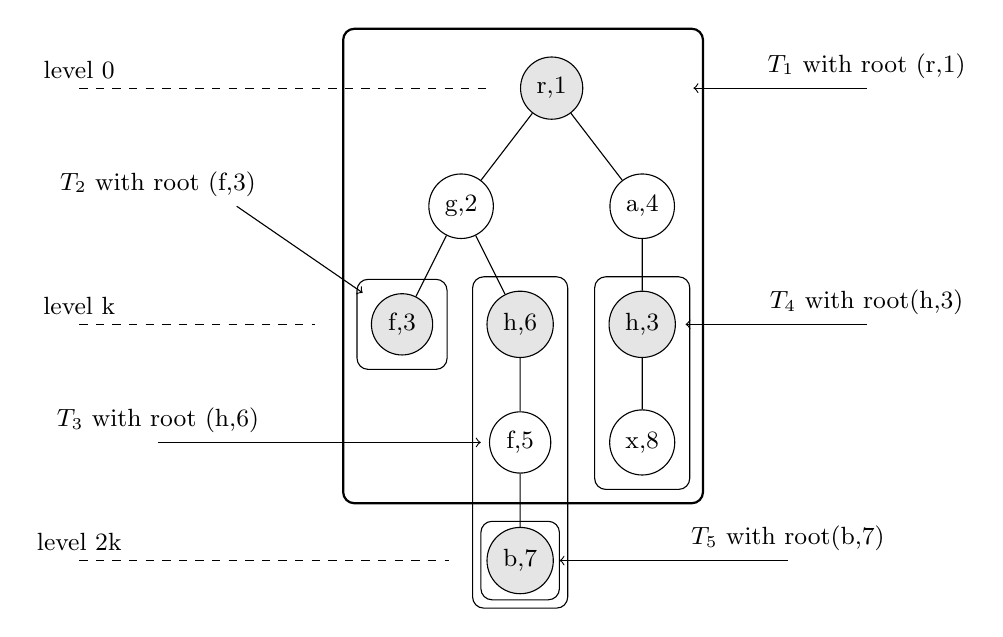
\begin{tikzpicture}[level distance=1.5cm,
  level 1/.style={sibling distance=2.3cm},
  level 2/.style={sibling distance=1.5cm},
  every node/.style={circle,draw,font=\small},
  knode/.style={fill=black!10},
  tnode/.style={above, draw=none, rectangle},
  every fit/.style = {draw, black, inner sep = 5pt, rectangle, rounded corners, thin}]
  
  \node (n0) [knode] at (0,0) {r,1}
  child { 
		node {g,2}
		child {node (n4) [knode] {f,3}}
		child {node (n1) [knode]  {h,6}
			child { node (n2) {f,5}
				child { node [knode] (n3) {b,7} }
			}
		}
  }
  child { node {a,4}
		child { node (n5) [knode] {h,3} 
			child { node (n6) {x,8} }
		}
  };

\node[fit=(n1) (n2) (n3)] {};
\node[fit=(n4)] {};
\node[fit=(n5) (n6)] {};
\node[fit=(n3), inner sep=2pt ] {};
\node[fit=(n0) (n2) (n6) (n4), inner sep=10pt, thick] {};

\draw [dashed] (-6,0) -- (-0.8,0) node [tnode, at start] {level 0};
\draw [dashed] (-6,-3) -- (-3,-3) node [tnode, at start]  {level k};
\draw [dashed] (-6,-6) -- (-1.3,-6) node [tnode, at start] {level 2k};

\draw [<-] (1.8,0) -- (4,0) node[tnode] {$T_1$ with root (r,1)};
\draw [->] (-4,-1.5) -- (-2.4,-2.6) node[tnode] at (-5, -1.5) {$T_2$ with root (f,3)};
\draw [->] (-5, -4.5) -- (-0.9, -4.5) node[tnode, at start] {$T_3$ with root (h,6)};
\draw [<-] (1.7, -3) -- (4, -3) node[tnode] {$T_4$ with root(h,3)};
\draw [<-] (0.1, -6) -- (3, -6) node[tnode] {$T_5$ with root(b,7)};
\end{tikzpicture}
}
\end{center}

\caption{A CCT with its $k$-level subtrees in evidence}
\label{cct2}
\end{figure}

Figure~\ref{cct2} illustrates a CCT and all its 5 subtrees at levels multiple of $k=2$.
Now, the $2$-SF of this CCT can be obtained by computing \texttt{join}($T_1$,\dots,$T_5$).
As fig.~\ref{ksf1} shows, the result is a forest with 4 trees: the first one is exactly $T_1$ because no other subtree has $r$ as root-label; the second one is that obtained by \texttt{join}($T_3$,$T_4$) and then last two ones are the one-node trees $T_2$ and $T_5$ which have not been joined because of their unique root-labels.

\begin{figure}[h]

\begin{center}
\scalebox{0.8}{

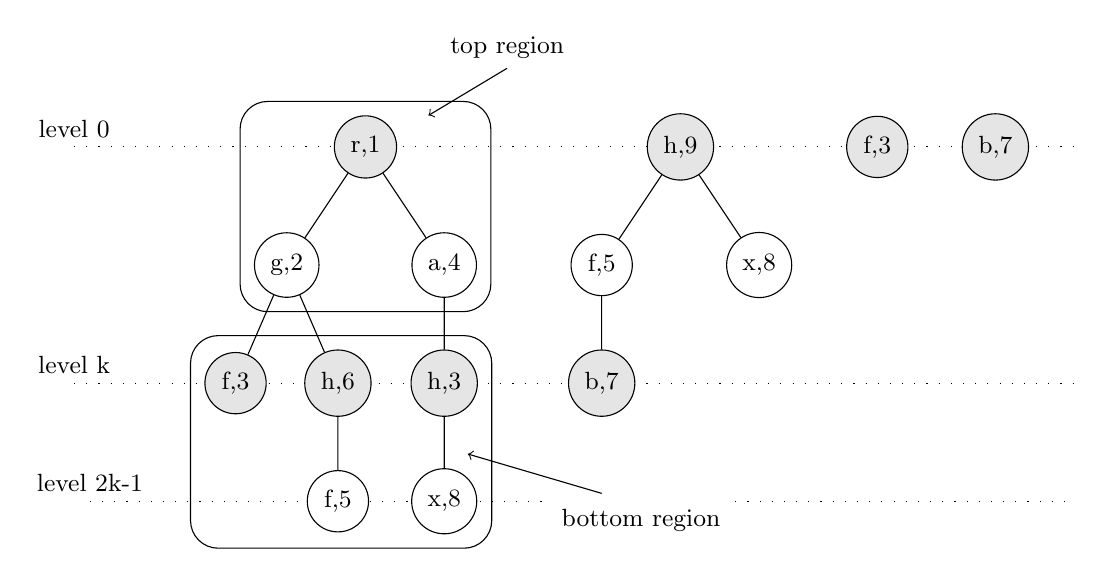
\begin{tikzpicture}[level distance=1.5cm,
  level 1/.style={sibling distance=2.0cm},
  level 2/.style={sibling distance=1.3cm},
  every node/.style={circle,draw,font=\small, radius=1, fill=white},
  knode/.style={fill=black!10},
  tnode/.style={above, draw=none, rectangle},
  every fit/.style = {draw, black, inner sep = 5pt, 
						rectangle, rounded corners=10pt, thin, fill=none}]
 
%\pgfdeclarelayer{back}
%\pgfsetlayers{back,main}

%\begin{pgfonlayer}{back}

\begin{scope}[on background layer]

\draw [loosely dotted] (-3.7,0) -- (9,0) node [tnode, at start] {level 0};
\draw [loosely dotted] (-3.7,-3) -- (9,-3) node [tnode, at start]  {level k};
\draw [loosely dotted] (-3.5,-4.5) -- (9,-4.5) node [tnode, at start] {level 2k-1};

\end{scope}
%\end{pgfonlayer}
 
  \node (n0) [knode] at (0,0) {r,1}
  child { 
		node (g2) {g,2}
		child {node (n4) [knode] {f,3}}
		child {node (n1) [knode]  {h,6}
			child { node (n2) {f,5} }
		}
  }
  child { node (a4) {a,4}
		child { node (n5) [knode] {h,3} 
			child { node (n6) {x,8} }
		}
  };

  \node [knode] at (4,0) {h,9}
  child { node {f,5} child { node [knode] {b,7} }}
  child { node {x,8} };

  \node [knode] at (6.5, 0) {f,3};
  \node [knode] at (8, 0) {b,7};

\node [fit = (n4) (n1) (n5) (n2) (n6)] {};
\node [fit = (n0) (g2) (a4)] {};

\draw [<-] (0.8,0.4) -- (1.8,1) node[tnode] {top region};
\draw [<-] (1.3,-3.9) -- (3, -4.4) node[tnode] at (3.5,-5) {bottom region};

\end{tikzpicture}
}
\end{center}

\caption{The $2$-SF relative to fig.~\ref{cct2}}
\label{ksf1}
\end{figure}

Now, $k$-SF has been defined and a way for building it from a CCT is shown but,
should be clear at this point that this method for building the $k$-SF is useless because
the $k$-CCF itself can be build directly from the CCT: the goal is to build $k$-SF \emph{without} a CCT and then to build the $k$-CCF from the $k$-SF. 

\subsection{Building a $k$-SF without a CCT}

The algorithm for building \emph{online} the $k$-SF is similar to the one purposed for building CCT but, instead of having 
one single \verb|currentNode| pointer (and, of course, only one tree), there two are pointers (\verb|top| and \verb|bottom|) that work at the same time on two different regions: \emph{top} region and \emph{bottom} region as shown in fig.~\ref{ksf1}.
Besides the two pointers and the $k$-SF, the algorithm uses:

\begin{itemize}
\item \verb|R|, a hashset which contains root pointers of all $k$-SF trees indexed by node label in a way that, given a label, it is possible to access its node-pointer in $O(1)$.

\item A shadow stack \verb|S| used for storing $\langle$top,bottom$\rangle$ pairs relative to each routine activation. 
\end{itemize}

At the algorithm start, \verb|S| contains a special pair of \verb|null| pointers; 
at the first procedure call, the \verb|if| condition on line 15 is verified:
the algorithm creates the root-node, makes \verb|top| pointing on it and adds also that pointer in \verb|R|. In the following procedure calls, the \verb|top| pointer is updated exactly as the \verb|currentNode| pointer in the CCT building algorithm (lines 36-46) except when \verb|S.size()-1| is a multiple of $k$: in that case (lines 16-34), \verb|bottom| is moved to \verb|top| and \verb|top| is moved to a (possibly) new tree of the forest; when the ``new'' tree already exists (this information is provided by \verb|R|), \verb|top| is simply moved to its root (line 25). After the first time \verb|top| is moved, the pointer \verb|bottom| is not more \verb|null| and is updated as the \verb|currentNode| pointer in CCT (lines 54-66). 

\begin{lstlisting}[language=java, label=ksf_alg, caption=An algorithm for building a $k$-SF,
			morekeywords={function,then,endif},
			frame=leftline,framesep=10pt,numbers=left, numbersep=15pt]

stack S
hashset R
forest kSF
node top=null,bottom=null

function init:
	S.push( (null,null) )

function func_call_event_handler(funcType func):

	(top,bottom) = S.top()
	
	/* update top region */
	if ( ( (S.size()-1) mod k ) == 0 ) then

		/* bottom is moved to top and top to a "new" tree */

		bottom=top
		node temp = R.find( func )

		if (temp == null) then

			/* a tree with label "func" does not exist */
			node n2 = new node( func, 0 )
			kSF.addTree(n2)
			R.add(n2)
			top=n2
		else

			/* a tree with label "func" already exists */
			top = temp
		endif

	else

		/* regular top pointer update */

		node temp = top.findNodeByFuncInChildren( func )

		if (temp == null) then
			temp = new node( func, 0 )
			top.addChildren( temp )
		endif

		top = temp

	endif

	top.incrementCounter()

	/* update bottom region */
	if (bottom != null) then
		
		/* regular bottom pointer update */

		node temp = bottom.findNodeByFuncInChildren( func )
		
		if (temp == null) then
			temp = new node( func, 0 )
			bottom.addChildren( temp )
		endif

		bottom = temp
		bottom.incrementCounter()

	endif

	/* top and bottom pointers are saved on the stack */
	S.push( (top, bottom) )

function func_ret_event_handler():

	/* 
		the last procedure returned, so its record 
		on the shadow stack is removed 
	*/
	
	S.pop()

\end{lstlisting}


\subsection{Building a $k$-CCF from a $k$-SF}

A $k$-CCF can be build from a $k$-SF using the following fundamental property of $k$-SF:
\begin{center}
$k$-CCF $=$ $inv_k$($k$-SF)
\end{center}
This means that a $k$-CCF can be obtained from a $k$-SF using the \emph{same} operation
used on a CCT, as if $k$-SF were a generalization of CCT: this is true and in fact, for $k\rightarrow \infty$, $k$-SF = CCT~\cite{kccf}.
There is only a problem in using the above property: the $k$-CCF build in that way has \emph{wrong} counters. The cause of that is the intrinsic data duplication in $k$-SF when a new tree is added by moving the \verb|top| pointer: \verb|top| and \verb|bottom| pointers build the same subtree in different places and both increment their counters. Of course, there is a solution: before applying $inv_k$ to $k$-SF, all counters of top regions of $k$-SF, except for the first tree, must be cleared to zero. The figure below shows that operation applied to the $k$-SF on fig.~\ref{ksf1}.


\begin{figure}[h]

\begin{center}
\scalebox{0.8}{

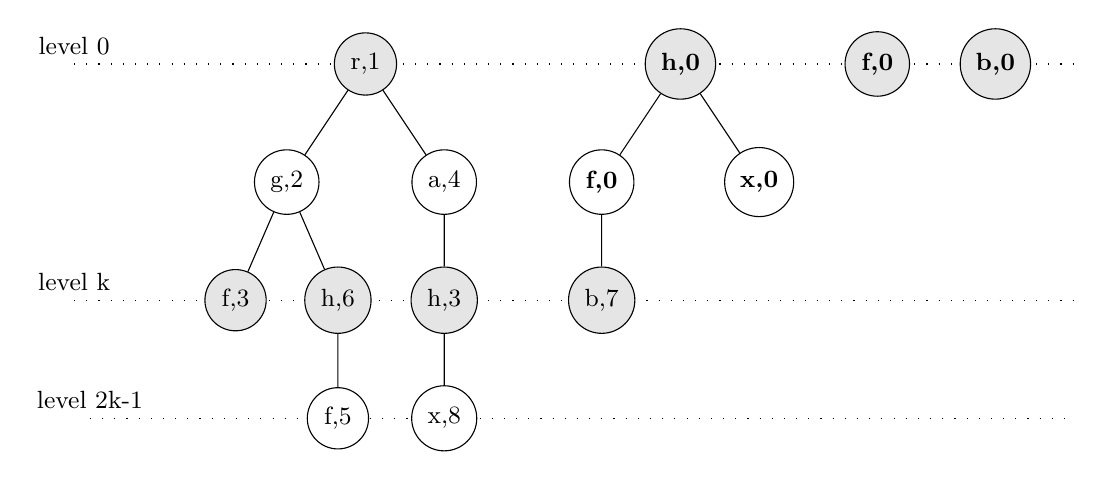
\begin{tikzpicture}[level distance=1.5cm,
  level 1/.style={sibling distance=2.0cm},
  level 2/.style={sibling distance=1.3cm},
  every node/.style={circle,draw,font=\small, radius=1, fill=white},
  knode/.style={fill=black!10},
  tnode/.style={above, draw=none, rectangle},
  every fit/.style = {draw, black, inner sep = 5pt, 
						rectangle, rounded corners=10pt, thin, fill=none}]
 
%\pgfdeclarelayer{back}
%\pgfsetlayers{back,main}

%\begin{pgfonlayer}{back}

\begin{scope}[on background layer]

\draw [loosely dotted] (-3.7,0) -- (9,0) node [tnode, at start] {level 0};
\draw [loosely dotted] (-3.7,-3) -- (9,-3) node [tnode, at start]  {level k};
\draw [loosely dotted] (-3.5,-4.5) -- (9,-4.5) node [tnode, at start] {level 2k-1};

\end{scope}
%\end{pgfonlayer}
 
  \node (n0) [knode] at (0,0) {r,1}
  child { 
		node (g2) {g,2}
		child {node (n4) [knode] {f,3}}
		child {node (n1) [knode]  {h,6}
			child { node (n2) {f,5} }
		}
  }
  child { node (a4) {a,4}
		child { node (n5) [knode] {h,3} 
			child { node (n6) {x,8} }
		}
  };

  \node [knode] at (4,0) {\textbf{h,0}}
  child { node {\textbf{f,0}} child { node [knode] {b,7} }}
  child { node {\textbf{x,0}} };

  \node [knode] at (6.5, 0) {\textbf{f,0}};
  \node [knode] at (8, 0) {\textbf{b,0}};

%\node [fit = (n4) (n1) (n5) (n2) (n6)] {};
%\node [fit = (n0) (g2) (a4)] {};

%\draw [<-] (0.8,0.4) -- (1.8,1) node[tnode] {top region};
%\draw [<-] (1.3,-3.9) -- (3, -4.4) node[tnode] at (3.5,-5) {bottom region};

\end{tikzpicture}
}
\end{center}

\caption{The $k$-SF of fig.~\ref{ksf1} with cleared counters in top regions}
\label{ksf2}
\end{figure}

\section{Final remarks}

In this chapter, $k$-CCF and $k$-SF data structures have been only \emph{basically} explained: many of their properties and theorems about them have been voluntarily omitted; 
also, no proofs neither any kind of space\slash time analysis have been shown.
This is because the goal of this chapter was only to explain what \emph{practically} $k$-CCF and $k$-SF are and how they can be \emph{technically} used in profilers such as IHPP. 

The author invites readers who really want to understand these data structures and their theoretical implications to read the original work \emph{k-Calling Context Profiling}~\cite{kccf}.


\chapter{An Intraprocedural Hot Path Profiler}

IHPP is a profiler written in C++. Technically it is not a program but
 a \emph{plug-in}\footnote{In the pin-specific slang,
plug-ins like IHPP are called \emph{pintools}.} for the tool 
Intel \textbf{Pin}\footnote{Official page: \url{http://www.pintool.org}}.
This last one, is a dynamic binary instrumentation framework for the IA-32 and x86-64 instruction-set architectures that allows the creation of dynamic program analysis tools. 
Pintools have, through pin, the full control of a target program: 
when this one is loaded in memory, all its routines and instructions are visible
to the pintool: it can modify or simply \emph{instrument} them. 
Instrumenting a routine means adding a \verb|call| instruction to a pintool analysis 
routine at its beginning; also, it is possible to instrument \verb|ret| instructions 
in order to catch \verb|return| statements of the target program: 
in this way a tool can build, for example, the program's CCT.
In this chapter, basics of IHPP such as its working modes and how can be used will be explained with a few technical considerations.

\section{An overview of IHPP}

IHPP has three main working modes: \emph{function}-mode, \emph{intra}-procedural mode and \emph{inter}-procedural mode. 

\begin{paragraph}{The function mode}
In this mode, IHPP builds a $k$-SF and a $k$-CCF for every thread of a program,
with an option (called \verb|joinThreads|) to join all $k$-SFs and produce a cumulative $k$-SF-$k$-CCF couple relative to the program execution.
This working mode is almost a direct application of the concepts explained in chapter 3. 
\end{paragraph}

\begin{paragraph}{The intra-procedural mode}
This other mode instead, deals with \emph{basic blocks} (from now called BBLs) inside procedures: the concept of \emph{calling a function} is transformed in the \emph{entering in a BBL}, while the concept of \emph{returning from a function call} totally disappears in this working mode; BBLs have no stack information and so, it is impossible to ``return'' to a previously activated BBL instance: it is only possible to activate this BBL again though a loop or a \verb|goto| statement.
IHPP instruments all BBLs inside chosen functions of a program and produces in output a couple $k$-SF-$k$-CCF for each function executed within each thread. The \verb|joinThreads| option is available also in this mode: it joins all $k$-SFs relative to a function generated by all threads in which that function has been called, for each function.
Another important feature in \emph{intra}-procedural mode is the \verb|rollLoops| option: it substantially produces $\infty$-SFs which do not grow due to loops inside functions because they are recognized and as result only counters are incremented. 
\end{paragraph}

\begin{paragraph}{The inter-procedural mode}
Despite of its name (\emph{intra}procedural profiler), IHPP has also a particular and unique working mode that deals with BBLs but in which the concept of \emph{procedure} is totally removed. In this working mode, a program is composed only by BBLs: there are no functions, so no calls and no returns. IHPP builds a couple of $k$-SF-$k$-CCF for each thread as other modes, but it is like the program has only one big procedure. This mode can be useful, for example, when one wants to analyze an algorithm implemented with two or more functions without considering the caller-callee relations but focusing the attention on execution flow of the hole algorithm. In the case when only one function is instrumented, even if it \emph{seems} that there is no difference between \emph{inter-} and \emph{intra-} procedural modes, in fact there is a \emph{big} difference: \emph{inter-}procedural mode ignores 
the function activation \emph{context} in which a basic block is activated. 
This concept will be, of course, explained later.
\end{paragraph}

\subsection{Technical considerations}

Like Pin itself, IHPP works both on Microsoft \textbf{Windows} and \textbf{Linux}-based systems but, output data sometimes is different and the reason is the compiler: 
under Linux systems the compiler \verb|gcc| is supported instead, under Windows only the compiler \verb|cl| included in the software \textbf{Visual Studio} is supported. 
This means that both the IHPP and the target program have to be compiled with the same compiler under a specific platform. Under Windows systems, target programs built with \verb|gcc| portings or other compilers are not supported due to problems with debug information: 
practically, IHPP fetches the debug information of a program through Pin which accepts only \verb|pdb| debug info format under Windows and only \verb|dwarf| format under Linux-based systems; but, the problematic difference between the two compilers is another: 
they compile C/C++ code in a different way and often they do not respect the \emph{standard calling conventions}, specially in auxiliary routines inserted into the target program. 
Because of this, a huge amount of work has been done in IHPP to overcome these problems, 
specially under Windows systems.

\section{The \emph{function} mode}

As said before, \emph{function} mode (internally called \verb|funcMode|) 
is a way of profiling very similar to the one theoretically explained in chapter 3.
A concrete example will be helpful to show this.

\begin{lstlisting}[language=C, 
	caption={prog1.c, a simple multi-threaded program}, 
	label=prog1, frame=leftline, numbers=left]

#include <stdio.h>
#include <stdlib.h>
#include <pthread.h>

void a(int x); void b(); void c();
void d(); void e(); void f();

void a(int x) { 

	if (!x) { 
		b(); c(); 
	} else { 
		b(); f();
	} 
}

void b() { }
void c() { }
void f() { }
void d() { c(); c(); }
void e() { d(); c(); a(0); }

void *thread2(void *arg) { a(1); return 0; }

int main(int argc, char ** argv) {

	int r;
	pthread_t th;

	a(0); e(); e();
	r = pthread_create(&th, NULL, thread2, NULL);
	pthread_join(th, NULL);
	return 0;
}

\end{lstlisting}

\noindent
Compiling the program in \cref{prog1} under a 32-bit Linux system with:
\begin{center}
\verb|gcc -g prog1.c -o prog1 -g -lpthread|
\end{center}
and starting IHPP analysis with\footnote{Due to permission problems under Linux pin have to be run with the \texttt{-injection child} option before the \texttt{-t} option. See its official user manual for an explanation.}:
\begin{center}
\begin{verbatim}
pin -t ihpp.so -ksf -kinf -funcMode -outfile out1.txt -- ./prog1
\end{verbatim}
\end{center}

will produce as output a file called \verb|out1.txt|\footnote{Some lines have been removed for compactness.}:

\begin{lstlisting}[label=out1, caption=file out1.txt]

K value: INFINITE
=============================================================================
Thread ID: 4294967296
=============================================================================
-----------------------------------------------------------------------------
DUMP of K-SF
-----------------------------------------------------------------------------
| _start(),1
   | __libc_csu_init(),1
      | __i686.get_pc_thunk.bx(),1
      | _init(),1
         | frame_dummy(),1
         | __do_global_ctors_aux(),1
   | main(),1
      | a(),1
         | b(),1
         | c(),1
      | e(),2
         | d(),2
            | c(),4
         | c(),2
         | a(),2
            | b(),2
            | c(),2
   | _fini(),1
      | __do_global_dtors_aux(),1
=============================================================================
Thread ID: 8589934593
=============================================================================
-----------------------------------------------------------------------------
DUMP of K-SF
-----------------------------------------------------------------------------

| thread2_func(),1
   | a(),1
      | b(),1
      | f(),1
\end{lstlisting}


A few considerations:
\renewcommand{\labelitemi}{$-$}

\begin{itemize*}
\item The program is multi-threaded and IHPP correctly shows this 
producing two different $k$-SFs. 
\item Only $k$-SFs are present in output because IHPP has been called without the \verb|-kccf| option.
\item $k$-SFs shown are in fact CCTs because \verb|-kinf| option is used.
\item The are some compiler routines that almost always will not be an object of interest for an user of IHPP. Note: programs compiled with \verb|cl| under Windows have \emph{hundreds} of compiler\slash library routines even if, of course, the program \emph{is not} compiled with \emph{static} linking of standard libraries. 
\end{itemize*}

\renewcommand{\labelitemi}{$\bullet$}
\noindent
Instead, executing IHPP on the same program but specifying this time the list 
of functions to instrument with \verb|-funcs a,b,c,d,e,f| the output written by IHPP is:

\begin{lstlisting}[label=out2, 
caption={The output of IHPP run with selective tracing}, frame=bottomline]
K value: INFINITE
=============================================================================
Thread ID: 4294967296
=============================================================================
-----------------------------------------------------------------------------
DUMP of K-SF
-----------------------------------------------------------------------------
| __root__(),1
   | a(),1
      | b(),1
      | c(),1
   | e(),2
      | d(),2
         | c(),4
      | c(),2
      | a(),2
         | b(),2
         | c(),2
=============================================================================
Thread ID: 8589934593
=============================================================================
-----------------------------------------------------------------------------
DUMP of K-SF
-----------------------------------------------------------------------------
| __root__(),1
   | a(),1
      | b(),1
      | f(),1
\end{lstlisting}
\noindent
It is clear that reading this output is easier than reading output in \cref{out1} but,
another thing comes out: there is \verb|__root__|, a ``new'' function not shown before.
It is not a really function but only a \emph{fake} symbol that IHPP automatically adds
as root of the first tree for each thread. The reason is simple: when an user specifies 
a list of functions, there is absolutely no guarantee that among these one is a relative root function.
One criticism towards this solution can be to say that $k$-SF is a \emph{forest}, not a tree, so the fake root node can be avoided: the answer is that criticism is wrong because of two reasons:
\begin{enumerate}
\item $\infty$-SF is a CCT \emph{by definition}: without the fake root $\infty$-SF will still be a forest and not a \emph{calling context tree}. 
\item Since $k$-SF will be wrong without a fake root (for all values of $k$ greater than a certain $\bar{k}$), a correct $k$-CCF could not be generated: as explained in chapter 3, before the $inv_k$ operation, counters of all nodes
in top regions must be cleared with the exception of the first three, which has as root node, the root of the CCT relative to the program execution trace. In the example above,
neither \verb|a()| nor \verb|e()| is eligible as CCT's root.
\end{enumerate}

\subsection{The \emph{joinThreads} option}

When invoking IHPP with the \verb|-joinThreads| option, after the target program ended
IHPP will join all $k$-SFs together before (eventually) building the $k$-CCF.
The output of IHPP after profiling the program in \cref{prog1} with this options is:

\begin{lstlisting}[label=out3, frame=bottomline, 
caption={the output of IHPP with the joinThreads option}]
-----------------------------------------------------------------------------
DUMP of K-SF
-----------------------------------------------------------------------------

| __root__(),2
   | a(),2
      | b(),2
      | c(),1
      | f(),1
   | e(),2
      | d(),2
         | c(),4
      | c(),2
      | a(),2
         | b(),2
         | c(),2
\end{lstlisting}
\noindent
Observing \cref{out3} should be clear that the $k$-SF of the second thread has been joined:
\verb|a()| and \verb|b()| counters of the first tree has been incremented and the \verb|f()| node has been added to the cumulative $k$-SF.

\subsection{The \emph{kccf} option}

Using the \verb|-kccf| option simply makes IHPP to produce also a $k$-CCF relative 
to each $k$-SF. It can be used with every value of $k$ specified by the option 
\verb|-k <value>| as it can used combined with the \verb|-kinf| even if this is often
useless. Below is shown the \emph{full} output of IHPP running on the program of \cref{prog1} with \verb|-joinThreads| \verb|-ksf| \verb|-kccf| \verb|-k 2| \verb|-funcs| \verb|a,b,c,d,e,f| options.
\begin{lstlisting}[label=out4, caption={a full IHPP output}, frame=bottomline]
K value: 2
Functions count: 18
Maximum number of different threads: 2
Nodes count of k slab forest: 20
Nodes count of kCCF: 25
-----------------------------------------------------------------------------
DUMP of K-SF
-----------------------------------------------------------------------------

| __root__(),2
   | a(),2
      | b(),2
      | c(),1
      | f(),1
   | e(),2
      | d(),2
         | c(),4
      | c(),2
      | a(),2
         | b(),2
         | c(),2
| b(),2
| c(),3
| d(),2
   | c(),4
| a(),2
   | b(),2
   | c(),2
| f(),1
-----------------------------------------------------------------------------
DUMP of K-CCF
-----------------------------------------------------------------------------

| __root__(),2
| a(),4
   | __root__(),2
   | e(),2
      | __root__(),2
| b(),4
   | a(),4
      | __root__(),2
      | e(),2
| c(),9
   | a(),3
      | __root__(),1
      | e(),2
   | d(),4
      | e(),4
   | e(),2
      | __root__(),2
| f(),1
   | a(),1
      | __root__(),1
| e(),2
   | __root__(),2
| d(),2
   | e(),2
      | __root__(),2
\end{lstlisting}

\noindent
Note: it is obvious that for finite values of $k$, IHPP produces as $k$-SF 
a \emph{real} forest and the fake node \verb|__root__| is the root \emph{only} of the first tree.

\subsection{The \emph{unrollSimpleRec} option}

Actually, with the options explained since now, IHPP does not produce an exactly standard
CCT or $k$-SF as a profiler which uses the algorithm for building a $k$-SF shown in chapter 3 will do. IHPP, by default, compresses (rolls) subtrees generated by recursions of single functions. \Cref{prog2} shows an appropriate example:

\begin{lstlisting}[language=C, 
	caption={prog2.c, a simple program that uses recursion}, 
	label=prog2, frame=leftline, numbers=left]

void foo(); void bar();

void recFunc(int n) {

	if (!n) { bar(); return; }
	recFunc(n-1);
}

void foo() { recFunc(5); }
void bar() { }

int main(int argc, char ** argv) { foo(); return 0; }

\end{lstlisting}

\noindent
The $\infty$-SF of program in \cref{prog2} produced by IHPP is:

\begin{lstlisting}[label=out5, caption={an example of $k$-SF \emph{without} the \texttt{unrollSimpleRec} option}, frame=bottomline]
| __root__(),1
   | main(),1
      | foo(),1
         | recFunc(),6
            | bar(),1
\end{lstlisting}

\noindent
It is clearly evident that recursion of \verb|recFunc()| is not explicitly shown.
Using the \verb|-unrollSimpleRec| option instead:
\begin{lstlisting}[label=out6, caption={an example of $k$-SF \emph{with} the \texttt{unrollSimpleRec} option}, frame=bottomline]
| __root__(),1
   | main(),1
      | foo(),1
         | recFunc(),1
            | recFunc(),1
               | recFunc(),1
                  | recFunc(),1
                     | recFunc(),1
                        | recFunc(),1
                           | bar(),1
\end{lstlisting}

\noindent
The output shown in \cref{out6} is the \emph{real} CCT of the program in \cref{prog2} 
but it is not more useful than the one in \cref{out5} even if it is longer: readers
would imagine what will happen if \verb|foo()| called \verb|recFunc()| with $n=10000$. 
Of course, using a finite value of $k$ will solve the problem but some information will be lost. An important consideration: when \verb|-unrollSimpleRec| is not used, \emph{only} 
recursions like the one just shown will be rolled, not the more complex recursions like 
those generated by the program in \cref{prog3}:

\begin{lstlisting}[language=C, 
	caption={prog3.c, a program that uses complex recursions}, label=prog3, 
	frame=leftline, numbers=left]

void bar(int n);

void foo(int n) {
	
	if (!n) return;
	bar(n-1);
}

void bar(int n) {

	if (!n) return;
	foo(n-1);
}

int main(int argc, char ** argv) { foo(5);	return 0; }

\end{lstlisting}

\noindent
Indeed, independently of the option \verb|-unrollSimpleRec|, 
IHPP produces this output for \verb|prog3|:
\begin{lstlisting}[label=out7, caption={IHPP partial output for \texttt{prog3}},frame=bottomline]
| __root__(),1
   | main(),1
      | foo(),1
         | bar(),1
            | foo(),1
               | bar(),1
                  | foo(),1
                     | bar(),1

\end{lstlisting}


\section{The \emph{intra}-procedural mode}

In the \emph{intra}-procedural mode (internally called \verb|intraMode|), 
IHPP traces BBLs (basic blocks) activations inside procedures building a couple $k$-SF-$k$-CCF for each procedure but, before proceeding, a BBL definition is necessary 
because the concept of BBL used in IHPP is a quite different from the classical one.

\subsection{The basic blocks}
The classical definition of BBL that can be found in textbooks is: \emph{a BBL is a single entrance, single exit sequence of instructions}. 
This definition can be perfectly applied to the concept of BBL used in IHPP, 
even if IHPP's BBLs are different from the classical ones. 
The following example will explain why.

\begin{lstlisting}[language=C, 
	caption={a switch statement}, label=switch, frame=leftline]

    switch(condition_var)
    {
        case 3: other_var++;
        case 2: other_var++;
        case 1: other_var++;
        case 0:
        default: break;
    }

\end{lstlisting}

\noindent
The \verb|switch| statement with fall-through cases in \cref{switch} 
will be usually compiled (for the IA-32 architecture) as something like this:

\begin{lstlisting}[language={[x86masm]Assembler}, 
	frame=leftline, label=asm1, caption={assembly code relative to \cref{switch}}]
.L10:
	add dword [ebp-4], 1
.L9:
	add dword [ebp-4], 1
.L8:
	add dword [ebp-4], 1
\end{lstlisting}

\noindent
According to the classical definition of BBL, \cref{asm1} contains three distinct BBLs, one for each instruction. Instead, in IHPP BBLs are still three but the first one, starting at \verb|.L10|, contains all the three instructions; the second one, starting at \verb|.L9|, contains the last two \verb|add| instructions and the last one is formed only by the 
last \verb|add| instruction. The reason of this different BBL concept is that 
IHPP is based on \textbf{Pin} and uses BBLs as provided by it. 
Pin, instead, has no way to ``extract'' classic BBLs from a compiled program because 
they can be only discovered at runtime: for example, when a branch (that could be indirect) sets the \emph{instruction pointer} to the second \verb|add| at \verb|.L9|, 
Pin has no way to know in advance that in the future (and this is not certain) some 
other branch will set the instruction pointer to \verb|.L8| so, the BBL starting at \verb|.L9| contains both \verb|add| instructions.

\subsection{\emph{Intra}Mode basics}

When run with the \verb|-intraMode| option, IHPP traces BBLs inside all functions or inside the chosen ones, like in the \emph{function} mode. Every BBL is identified in output by: 
\begin{itemize*}
\item the function's name which the BBL belongs to
\item the offset BBL address - function address in bytes
\item the line and the column of the first 
statement in program source code that belongs to the BBL\footnote{In order all this data to be obtained from the executable, it \emph{must} be build 
with debug info as told in the chapter's beginning: programs without debug info 
cannot be analyzed by IHPP, independently from the working mode.}.
\end{itemize*}

\Cref{prog4} shows a program that is going to be analyzed.

\begin{lstlisting}[language=C, 
	caption={prog4.c, another simple program}, label=prog4, frame=leftline, numbers=left]
#include <stdio.h>

void p(int n) { 
	
	printf("%d\n", n); 
}

void foo(int n) {

	int i;

	if (n) {

		p(0);

		for (i=0; i < 3; i++) {
			p(1);
		}

		foo(0);

	} else {
		p(2);
	}
}

int main(int argc, char ** argv) { foo(1); return 0; }
\end{lstlisting}

\noindent
Running IHPP with \verb|-intraMode -ksf -k 100 -funcs foo,p| produces:

\begin{lstlisting}[label=out8, caption={IHPP partial output for \texttt{prog4}},frame=bottomline]
=============================================================================
Function: p()
-----------------------------------------------------------------------------
DUMP of K-SF
-----------------------------------------------------------------------------
| {p+0 at 3,0},5
   | {p+26 at 6,0},5
=============================================================================
Function: foo()
-----------------------------------------------------------------------------
DUMP of K-SF
-----------------------------------------------------------------------------
| {foo+0 at 8,0},2
   | {foo+12 at 14,0},1
      | {foo+24 at 16,0},1
         | {foo+49 at 16,0},1
            | {foo+33 at 17,0},1
               | {foo+45 at 16,0},1
                  | {foo+33 at 17,0},1
                     | {foo+45 at 16,0},1
                        | {foo+33 at 17,0},1
                           | {foo+45 at 16,0},1
                              | {foo+55 at 20,0},1
                                 | {foo+67 at 20,0},1
                                    | {foo+81 at 25,0},1
   | {foo+69 at 23,0},1
      | {foo+81 at 25,0},1

\end{lstlisting}

\noindent
A few preliminary considerations about \cref{out8}:
\renewcommand{\labelitemi}{$-$}

\begin{itemize}
\item All column values are zero: this happens when 
column information is not available but it is not necessary a whole program 
problem: some BBLs could have this info and others could not, depending from the compiler.
\item In this example, as in many others, only $k$-SFs with big values of $k$
are shown because they provide full information analysis. This approach is the best for 
simple programs which practically allows it. 
But, in this particular example these is a specific reason to use $k=100$ instead of $k=\infty$: IHPP does not allow \verb|-kinf| option alone in \emph{intra}Mode because
output size is potentially unbounded. The only way for using \verb|-kinf| option is combined with \verb|-rollLoops| which will be explained later.
\end{itemize}
\renewcommand{\labelitemi}{$\bullet$}

\begin{paragraph}{An interpretation}
Comparing the output in \cref{out8} with the program in \cref{prog4} it is possible to 
observe a good matching between them, for example, the loop in lines 16-17 
is clearly visible; also, the behavior of the \verb|if-then-else| statement in \verb|foo()| is evident. In particular, recognizing this last one is not trivial: 
IHPP has to understand that a recursion has occurred and lines 23-25
are not executed after line 20 but instead, in a new function activation. 
From a theoretically point of view, 
this is \emph{equivalent} to building a different $k$-SF
for \emph{each} function activation and then joining all them. 
Practically, IHPP achieves it in a better way: 
it substantially uses a \emph{shadow stack} to trace function activations in which
a couple of pointers (\verb|top|,\verb|bottom|) [see chapter 3] is stored for each 
function activation. Details of this approach will be explained in the next chapter.
\end{paragraph}

Attentive readers will have probably noticed that there are two BBLs on line 16 
and other two ones on line 20: even if it is clear that they are distinct 
BBLs due to their function offset, it is not obvious what they exactly do.
Since there is no other way than looking machine instructions to understand 
what a BBL do, IHPP provides an option to do this.

\subsection{Inside a BBL: the disassembly utility in IHPP}

Using the option \verb|-blocksDisasm| together with the option \verb|-showBlocks| 
when calling IHPP, makes it to write at the of the output file a table 
that contains for each BBL, four columns: its string name (used in $k$-SFs), its memory address, the absolute number of times it has been called (vertex profiling) and
a kind of ``special'' disassembly. This last column is a post-elaborated form 
of the Intel-style disassembly that Pin provides to IHPP: usually in disassembly 
no labels are used in call and branch instructions and they appear something like this: 
\verb|jle 0x8048400|. IHPP, in order to help the analyst who uses it, replaces 
all addresses with human readable strings. The \cref{out9} shows that.

\begin{lstlisting}[language={[x86masm]Assembler}, 
	label=out9, caption={a part of ``all basic blocks'' table}, frame=bottomline]

-----------------------------------------------------------------------------
All basic blocks
-----------------------------------------------------------------------------


{foo+24 at 16,0} addr: 0x8048418 counter: 1	
Disassembly: 
											mov dword ptr [ebp-0xc], 0x0
											jmp {foo+49 at 16,0}

{foo+33 at 17,0} addr: 0x8048421 counter: 3	
Disassembly: 
											mov dword ptr [esp], 0x1
											call p

{foo+45 at 16,0} addr: 0x804842d counter: 3	
Disassembly: 
											add dword ptr [ebp-0xc], 0x1
											cmp dword ptr [ebp-0xc], 0x2
											jle {foo+33 at 17,0}

{foo+49 at 16,0} addr: 0x8048431 counter: 1	
Disassembly: 
											cmp dword ptr [ebp-0xc], 0x2
											jle {foo+33 at 17,0}

{foo+55 at 20,0} addr: 0x8048437 counter: 1	
Disassembly: 
											mov dword ptr [esp], 0x0
											call foo

{foo+67 at 20,0} addr: 0x8048443 counter: 1	
Disassembly: 
											jmp {foo+81 at 25,0}

\end{lstlisting}

Observing the \cref{out9}, the reason why there are two BBLs on line 16 comes out:
the BBL at \verb|foo+24| is the \verb|i=0| initialization statement 
of the \verb|for| loop, instead, the BBL at \verb|foo+45| contains the \verb|i++| statement and a conditional branch (which makes the loop to continue) taken when
\verb|i <= 2|. In this case, as it happens very often, machine instructions 
do not follow the order of \verb|C| statements. BBLs on line 20 instead, are contiguous
but are separated due to a \verb|call| instruction at the end of the first one.

\begin{paragraph}{Advanced features}
The IHPP disassembly system has an advanced feature not shown in \cref{out9}.
Analyzing the program in \cref{prog4} with IHPP with under Windows 
systems\footnote{The program have to be compiled with the Visual Studio's \texttt{cl} 
compiler using the option \texttt{\slash Wi} to enable debug info generation},
the disassembly code relative to the Linux BBL \verb|{foo+55 at 20,0}| is:
\begin{lstlisting}[language={[x86masm]Assembler}, 
	label=out10, caption={an example of an indirect call}, frame=bottomline]

{foo+68 at 23,0} addr: 0x951094 counter: 1	
Disassembly: 
										push 0x1
										call .text+5 --> jmp {p+0 at 3,0}
\end{lstlisting}

This means that \verb|foo()| does not call \verb|p()| function \emph{directly}, 
but instead it calls an \emph{undefined} area of the \verb|.text| section of the program situated five bytes from the beginning; in this location, a direct jump instruction
makes the program to run the \verb|p()| routine. Since practically all user functions
are called in this indirect way when compiling with \verb|cl| programs with debug info,
the implementation of this feature was strictly necessary. IHPP can handle also
the hypothetical situation in which a call is done through two or more indirect jumps.
\end{paragraph}

\begin{paragraph}{The full disassembly of routines}
IHPP offers also the opportunity to show at the end of the output file 
a table containing all routines using the option \verb|-showFuncs| and their 
disassembly code adding also the \verb|-funcsDisasm| option.  
In \emph{intra-} and \emph{inter-} procedural modes, both options (\verb|showFuncs| and \verb|showBlocks|) can be used, instead, in \emph{function} mode only \verb|showFuncs| can be used.
\end{paragraph}

\subsection{The \emph{rollLoops} option}

Running IHPP with the \verb|-rollLoops| option on the program in the \cref{prog4}
produces for the \verb|foo()| function the $k$-SF in the \cref{out10}:

\begin{lstlisting}[label=out10, caption={an output of IHPP with rollLoops option}]
-----------------------------------------------------------------------------
| {foo+0 at 8,0},2
   | {foo+12 at 14,0},1
      | {foo+24 at 16,0},1
         | {foo+49 at 16,0},1
            | {foo+33 at 17,0},3
               | {foo+45 at 16,0},3
                  | {foo+55 at 20,0},1
                     | {foo+67 at 20,0},1
                        | {foo+81 at 25,0},1
   | {foo+69 at 23,0},1
      | {foo+81 at 25,0},1
\end{lstlisting}

It is clearly visible that the \verb|for| loop on lines 16-17 
has been compressed or, in specific slang, \emph{rolled}.
The \verb|-rollLoops| option, as told before, implies the \verb|-kinf| option
that means $k=\infty$ but, the output size is always limited.

\subsection{The \emph{joinThreads} option in \emph{intraMode}}

The concept of the \verb|-joinThreads| option is the same as in the 
\emph{function} mode even if an example will make it clear. 

\begin{lstlisting}[language=C, 
	caption={prog5.c, an example program}, label=prog5, frame=leftline, numbers=left]
#include <stdio.h>
#include <stdlib.h>
#include <pthread.h>

void *foo(void *arg) {

	int i=0;

	while(1) {

		if (arg) {
		
			if (i >= 3)
				break;	
		} else {

			if (i >= 9)
				break;
		}
		
		printf("%i\n",i);
		i++;
	}

	return 0;
}

int main(int argc, char ** argv) {

	pthread_t th;
	
	foo((void*)1);

	pthread_create(&th, NULL, foo, NULL);
	pthread_join(th, NULL);

	return 0;
}

\end{lstlisting}

\noindent
The IHPP analysis of the program in \cref{prog5} with the options\\\verb|-intraMode| \verb|-rollLoops| \verb|-func foo| produces the following output\footnote{A great deal of output lines have been omitted}:

\begin{lstlisting}[label=out11, caption={the output of IHPP analyzing \texttt{prog5}}]
=============================================================================
Thread ID: 4294967296
=============================================================================

| {foo+0 at 5,0},1
   | {foo+19 at 13,0},4
      | {foo+33 at 21,0},3
         | {foo+53 at 22,0},3
            | {foo+13 at 11,0},3
      | {foo+25 at 14,0},1
         | {foo+60 at 25,0},1

=============================================================================
Thread ID: 8589934593
=============================================================================

| {foo+0 at 5,0},1
   | {foo+27 at 17,0},10
      | {foo+33 at 21,0},9
         | {foo+53 at 22,0},9
            | {foo+13 at 11,0},9
      | {foo+59 at 18,0},1

\end{lstlisting}

\noindent
Instead, using the \verb|-joinThreads| option, the output is:

\begin{lstlisting}[label=out12, 
caption={the output of IHPP analyzing \texttt{prog5} with \texttt{-joinThreads}}]
=============================================================================
Function: foo()
=============================================================================
| {foo+0 at 5,0},2
   | {foo+19 at 13,0},4
      | {foo+33 at 21,0},3
         | {foo+53 at 22,0},3
            | {foo+13 at 11,0},3
      | {foo+25 at 14,0},1
         | {foo+60 at 25,0},1
   | {foo+27 at 17,0},10
      | {foo+33 at 21,0},9
         | {foo+53 at 22,0},9
            | {foo+13 at 11,0},9
      | {foo+59 at 18,0},1

\end{lstlisting}

\noindent
Even if the interpretation of the outputs at the point \emph{should} be trivial,
some complications not correlated with the \emph{joinThreads} option 
has came out.
The function \verb|foo()| is executed once per thread; in the main thread, the loop does 3 iterations and then exists going to line 14, instead
in the second one, the loop does 9 iterations and then exists going to line 18.
A first problem: it is unclear why BBL at line 11 is activated \emph{after} 
and not \emph{before} BBL at line 22. The answer can be found only by looking at
the disassembly code in \cref{intraJoinThAsm}.

\begin{lstlisting}[language={[x86masm]Assembler}, 
	label=intraJoinThAsm, caption={a part of ``all basic blocks'' table of \texttt{prog5}}]

{foo+0 at 5,0} addr: 0x80484c4 counter: 2   
Disassembly:
												push ebp
												mov ebp, esp
												sub esp, 0x28
												mov dword ptr [ebp-0xc], 0x0
												cmp dword ptr [ebp+0x8], 0x0
												jz {foo+27 at 17,0}
{foo+13 at 11,0} addr: 0x80484d1 counter: 12
Disassembly: 
												cmp dword ptr [ebp+0x8], 0x0
												jz {foo+27 at 17,0}

{foo+19 at 13,0} addr: 0x80484d7 counter: 4
Disassembly: 
												cmp dword ptr [ebp-0xc], 0x2
												jle {foo+33 at 21,0}

{foo+25 at 14,0} addr: 0x80484dd counter: 1
Disassembly: 
												jmp {foo+60 at 25,0}

{foo+27 at 17,0} addr: 0x80484df counter: 10
Disassembly: 
												cmp dword ptr [ebp-0xc], 0x8
												jnle {foo+59 at 18,0}

{foo+59 at 18,0} addr: 0x80484ff counter: 1
Disassembly: 
												nop 
												mov eax, 0x0
												leave 
												ret 

{foo+60 at 25,0} addr: 0x8048500 counter: 1 
Disassembly: 
												mov eax, 0x0
												leave 
												ret 

\end{lstlisting}

The BBL \verb|{foo+0 at 5,0}| includes in itself the BBL \verb|{foo+13 at 11,0}|: 
that is the reason why BBL on line 11 is not activated suddenly 
after the BBL on line 5; instead, it is activated at every loop iteration 
after BBL on line 22 (not shown in the \cref{intraJoinThAsm}). 
The same ``problem'' occurs for BBLs on lines 18 and 25: 
as already explained, the origin of this unusual concept of BBL is the real-time BBL 
identification: when the program ran at \verb|foo+13| (included in BBL at \verb|foo+0|),
\textbf{Pin} had no way to understand that in the future a BBL at \verb|foo+53| will 
branch to it.

Apart of these considerations about BBLs, as it can be seen in \cref{out12},
the behavior of the \emph{joinThreads} option is exactly what one expects: 
it produces as output the forest join of the $k$-SFs related to each thread, 
or better, in this particular case, the \emph{tree} join of the two CCTs.

\section{The \emph{inter}-procedural mode}

When launched with the \verb|-intraMode| option\footnote{The inter-procedural mode is often called internally in IHPP \texttt{interProcMode} instead of \texttt{interMode} to 
avoid misunderstanding problems correlated with \texttt{intraMode}.}
, IHPP instruments only BBLs 
and builds \emph{inter}-procedural $k$-SFs, one for each thread. 
Each $k$-SF, contains BBLs which belong to chosen functions or, eventually, to all 
functions of the main image of the target program. The below listings show 
an example program and its relative IHPP analysis output for $k=100$.

\begin{lstlisting}[language=C, 
	caption={prog6.c, an example program}, label=prog6, frame=leftline, numbers=left]
void bar(int n); void f3() { }

void foo() { 

	bar(0); 
	f3(); 
	bar(1); 
}

void bar(int n) { 

	if (n) 
		f3(); 
}
int main(int argc, char ** argv) { foo(); return 0; }
\end{lstlisting}

\begin{lstlisting}[label=out13, 
caption={partial output of IHPP analysis in \texttt{interProcMode} of \texttt{prog6}}]

| {__root__+0 at 0,0},1
   | {foo+0 at 3,0},1
      | {bar+0 at 10,0},1
         | {bar+14 at 14,0},1
            | {foo+18 at 6,0},1
               | {f3+0 at 1,0},1
                  | {foo+23 at 7,0},1
                     | {bar+0 at 10,0},1
                        | {bar+9 at 13,0},1
                           | {f3+0 at 1,0},1
                              | {bar+14 at 14,0},1
                                 | {foo+35 at 8,0},1

\end{lstlisting}

Observing output in \cref{out13} should be enough to understand what the 
\emph{inter}-procedural mode does: a $k$-SF is build as if there were no routines at all.
An important consideration about this IHPP working mode is that even if
only one produce is instrumented, the output will be different to the one made by 
\verb|intraMode|; a proof for this is given by \cref{out14} which shows
the IHPP analysis output of program in \cref{prog4}, 
already analyzed in \verb|intraMode| in the \cref{out8}.

\begin{lstlisting}[label=out14, 
caption={partial output of IHPP analysis in \texttt{interProcMode} of \texttt{prog4}}]
-----------------------------------------------------------------------------
DUMP of K-SF
-----------------------------------------------------------------------------

| {__root__+0 at 0,0},1
   | {foo+0 at 8,0},1
      | {foo+12 at 14,0},1
         | {foo+24 at 16,0},1
            | {foo+49 at 16,0},1
               | {foo+33 at 17,0},1
                  | {foo+45 at 16,0},1
                     | {foo+33 at 17,0},1
                        | {foo+45 at 16,0},1
                           | {foo+33 at 17,0},1
                              | {foo+45 at 16,0},1
                                 | {foo+55 at 20,0},1
                                    | {foo+0 at 8,0},1
                                       | {foo+69 at 23,0},1
                                          | {foo+81 at 25,0},1
                                             | {foo+67 at 20,0},1
                                                | {foo+81 at 25,0},1

\end{lstlisting}

\noindent
It is evident that the recursion of \verb|foo()| has absolutely no effect:
the BBL \verb|{foo+0 at 8,0}| follows the BBL \verb|{foo+55 at 20,0}| as if 
it was a simply loop iteration.

A last note: IHPP supports also \emph{rollLoops} and \emph{joinThreads} options
in \verb|interProcMode|, even if no examples are provided here.

\section{The \emph{XML} output feature}

IHPP has been designed to be \emph{extensible} and since data exchange is on the basis
of that principle, IHPP provides an alternative output format.

Using the \verb|-xml| option, IHPP will provide its output in \textbf{XML} format
which is nowadays one of most supported data exchange languages.
The IHPP-specific XML language is defined in a computer interpretable form too, 
using the \textbf{XML Schema} language. 
The specific \textbf{XSD} file that contains the output language definition 
is called \verb|outputschema.xsd| and it is located in the \verb|doc/| directory
of the project.

\chapter{The implementation}

Actually, the IHPP project is written in about 4,800 lines of \verb|C++| 
code\footnote{All source code line are included in this calculation, even ones which 
contain comments and the empty ones.}: 
even only copying down its full source code will take about 82 pages using
this font. Therefore, the goal of this chapter is not to explain 
all IHPP source code line by line, but instead is to give to the reader 
a panoramic overview of the project implementation, showing its architecture, 
its key-files and the approaches adopted for solving problems occurred.
Of course, there will be source code listings, but almost always the code will be
\emph{purged} from the lines unessential for specific context in which the code is presented.

\section{A general overview of the project}

As can be seen in \cref{proj_files}, IHPP has been implemented in 26 files,
grouped by areas of competence. The \verb|main.cpp| file is where the enter point
 of the profiler is located and contains, in addition to the initialization code, all \emph{instrumentation routines}. These last ones substantially place \emph{callbacks}
in the target program to functions located in files of group (3): functions in these
files use context objects defined in files of groups (4), 
tracing objects defined in files of group (2) and specially
the \verb|traceObject()| function implemented in \verb|traceObjFunc.cpp|.
This last one, is substantially the function that implements the algorithm for building
a $k$-SF from an execution trace shown in \cref{ksf_alg}: 
when called, it \emph{traces} the activation of a generic \verb|TracingObject<T>| 
in the given \emph{context}. The \emph{context} depends from the working mode:
in \verb|funcMode|, for example, the \emph{context} is pointer to a \verb|ThreadContext| object; instead, in \verb|IntraMode| the \emph{context} is 
a pointer to a \verb|IntraModeContext| object. In order to simply everything, 
\emph{abstraction} is used: 
both \verb|ThreadContext| and \verb|IntraModeContext| classes
are specializations of
the \verb|GenericTraceContext| class, exactly as \verb|FunctionObj| and 
\verb|BasicBlock| classes are specializations of the generic \verb|TracingObject<T>| class.
\begin{figure}[H]

%\begin{center}
%\scalebox{1.0}{

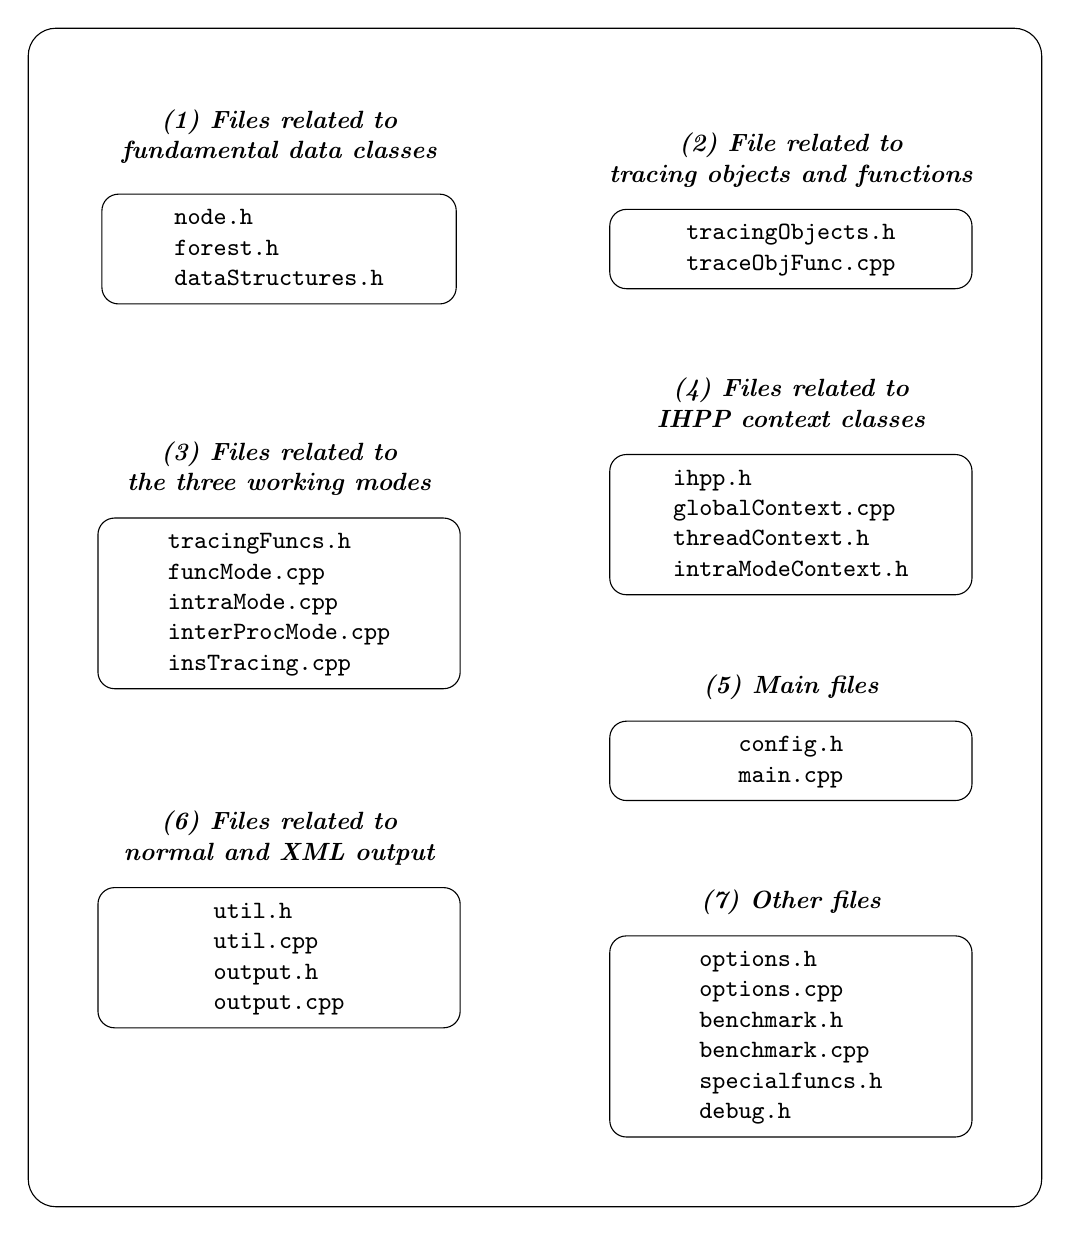
\begin{tikzpicture}
[
flist/.style = {rectangle, rounded corners=6pt, 
					thin, draw, font=\small\ttfamily, minimum width = 4.6cm},
headnode/.style = {rectangle, fill=none, font=\small\bfseries\itshape}
]

%\begin{scope}[shift={(-5cm,0)}]

\node[flist, minimum width = 4.5cm] (n1) at (0,0) {
\makecell[l]{
node.h\\
forest.h\\
dataStructures.h
}};

\node[headnode, above = 0.2cm of n1] (t1) { 
\makecell[c] {
(1) Files related to\\ 
fundamental data classes 
}};

\node[flist] (n2) at (6.5,0) {
\makecell[l] {
tracingObjects.h\\
traceObjFunc.cpp
}};

\node[headnode, above = 0.1cm of n2] (t2) {
\makecell[c] {
(2) File related to\\
tracing objects and functions
}};

\node[flist] (n3) at (0,-4.5) {
\makecell[l] {
tracingFuncs.h\\
funcMode.cpp\\
intraMode.cpp\\
interProcMode.cpp\\
insTracing.cpp
}};

\node[headnode, above = 0.1cm of n3] (t3) {
\makecell[c] {
(3) Files related to\\
the three working modes
}};

\node[flist] (n4) at (6.5,-3.5) {
\makecell[l] {
ihpp.h\\
globalContext.cpp\\
threadContext.h\\
intraModeContext.h
}};

\node[headnode, above = 0.1cm of n4] (t4) {
\makecell[c] {
(4) Files related to\\
IHPP context classes
}};

\node[flist] (n5) at (6.5,-6.5) {
\makecell[l] {
config.h\\
main.cpp
}};

\node[headnode, above = 0.1cm of n5] (t5) {
\makecell[c] {
(5) Main files
}};

\node[flist] (n6) at (0,-9) {
\makecell[l] {
util.h\\
util.cpp\\
output.h\\
output.cpp
}};

\node[headnode, above = 0.1cm of n6] (t6) {
\makecell[c] {
(6) Files related to\\
normal and XML output
}};

\node[flist] (n7) at (6.5,-10) {
\makecell[l] {
options.h\\
options.cpp\\
benchmark.h\\
benchmark.cpp\\
specialfuncs.h\\
debug.h
}};

\node[headnode, above = 0.1cm of n7] (t7) {
\makecell[c] {
(7) Other files
}};

\node[rectangle, thin, draw, inner sep = 25pt, 
rounded corners = 10pt, fit = (t1) (n2) (n6) (n7)] {};

%\draw[thin, rounded corners = 10pt] (-3.5,2.5) rectangle +(14,-15);

%\end{scope}

\end{tikzpicture}

%}
%\end{center}

\caption{File organization of the project}
\label{proj_files}

\end{figure}

\noindent 
The \verb|traceObject()| function mentioned before, works with basilar objects 
defined in files of group (1). The first two files in this last group use on their basis
container classes for \verb|ObjectWithKey<T>| objects defined and implemented 
in file \verb|dataStructures.h|.
\verb|ObjectWithKey<T>| is the most abstract class in IHPP since it is a generalization of the abstract class \verb|TracingObject<T>|. 
Nodes and forests data structures are implemented respectively in \verb|node.h| and \verb|forest.h| files. The concept of \emph{tree} is not explicitly modeled in IHPP, but it is 
modeled inside the \verb|node<T>| class instead. 
\begin{paragraph}{A technical note}
Files in groups (1) and (2) 
are mainly \emph{headers} because they
contain \emph{template} classes which cannot be complied like others; 
the \verb|traceObject()| function instead, is not a template function because of 
an optimization strategy: it is a function pointer which is assigned at runtime
to the \emph{faster} \verb|traceObject| implementation, specially to speeding up 
the $k=\infty$ case. 
\end{paragraph}

\Cref{classdiag1} shows an UML-like diagram which summarizes
some of the relations just explained.

\begin{figure}[h]

\begin{center}

\scalebox{0.9} {
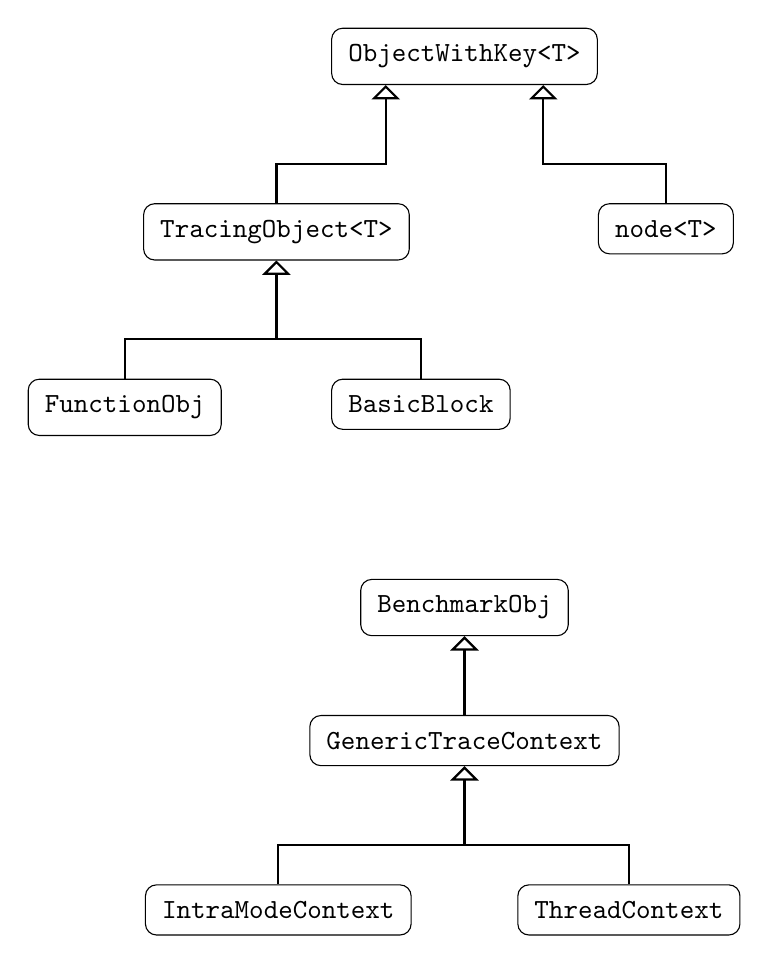
\begin{tikzpicture}
[
	class/.style = {rectangle, draw, rounded corners = 4pt, inner sep=6pt, font=\ttfamily},
	arrow/.style = {->, >=open triangle 90, thick},
	line/.style = {-, thick}
]

\node[class] (objectwithkey) at (0,0) {ObjectWithKey<T>};
\node[class, below left = 1.5cm and -1cm of objectwithkey] (tracingobject) {TracingObject<T>};
\node[class, below left = 1.5cm and -1cm of tracingobject] (functionobj) {FunctionObj};
\node[class, below right = 1.5cm and -1cm of tracingobject] (basicblock) {BasicBlock};

\node[class, below right = 1.5cm and 0cm of objectwithkey] (nodet) {node<T>};

\draw[arrow] (tracingobject.north) -- ++(0,0.5) -| ([xshift=-1cm] objectwithkey.south);
\draw[arrow] (functionobj.north) -- ++(0,0.5) -| (tracingobject.south);
\draw[line, shorten >= 0.5cm] (basicblock.north) -- ++(0,0.5) -| (tracingobject.south);

\node[class] (bench) at (0,-7) {BenchmarkObj};
\node[class, below = of bench] (genericCtx) {GenericTraceContext};
\node[class, below left = 1.5cm and -1.3cm of genericCtx] (intraCtx) {IntraModeContext};
\node[class, below right = 1.5cm and -1.3cm of genericCtx] (thCtx) {ThreadContext};

\draw[arrow] (genericCtx.north) -- ++(0,0) -| (bench.south);
\draw[arrow] (intraCtx.north) -- ++(0,0.5) -| (genericCtx.south);
\draw[line, shorten >= 0.5cm] (thCtx.north) - ++(0,0.5) -| (genericCtx.south);
\draw[arrow] (nodet.north) -- ++(0,0.5) -| ([xshift=1cm] objectwithkey.south);

\end{tikzpicture}
}

\end{center}

\caption{some important class relationships}
\label{classdiag1}
\end{figure}

\begin{paragraph}{The output generation}
When the target program ends, the \verb|Fini()| \emph{callback} routine located in 
\verb|output.cpp| is called. It writes the output, as shown in chapter 4, using 
supporting routines in \verb|output.cpp| and \verb|util.cpp| files.
When the \verb|-kccf| option is used, supporting routines in \verb|output.cpp| 
use the \verb|inverseK()| method of class \verb|forest<T>| to produce a $k$-CCF
from each $k$-SF. The \verb|-joinThreads| option makes output routines to 
do a preventive \emph{join} operation on all $k$-SFs, leaving the result 
in the first thread context. 
\end{paragraph}

\begin{paragraph}{The \emph{instruction} tracing mode}
The shortly called \emph{insTracing} mode is a hidden part of IHPP never
mentioned before. It handles the instrumenting of \emph{all} machine instructions
contained in chosen functions in order to improve correctness 
of outputs produced by \verb|funcMode| and \verb|intraMode| 
in \emph{extreme} conditions, for example when \emph{calling conventions} are not
respected by the compiler such as a call to routine with a \verb|jmp| instruction 
instead of a \verb|call| one, or when particular functions like \verb|longjmp()| are used.
This \emph{feature} consists of a \emph{set} of several approaches to the problem 
of correctly understanding the execution trace of the program but, 
since it is really \emph{heavier} than the simply function instrumentation,
it can be disabled (each approach separately) in the \verb|config.h| file.
\end{paragraph}

\begin{paragraph}{Other features}
IHPP has implemented in it a tiny benchmark framework which allows 
to count the number of nodes and forests created and copied (during the 
target program execution) within each
thread or even each function in each thread. For that reason,
the \verb|GenericTraceContext| class derives from the \verb|BenchmarkObj| class.
Of course, benchmark is a \emph{heavy} feature too which can be disabled 
in the \verb|config.h| file. Also, IHPP provides a set \emph{debug} mode
which writes selective debug info to the \verb|stderr| file stream.
\end{paragraph}

\section{The context classes}

The knowledge of context classes is essential to understand the IHPP implementation.

\subsection{The \emph{GlobalContext} class}
The main IHPP context class is \verb|GlobalContext|: it contains all globally shared variables in the program and it is instanced only once. 
Even if the \emph{singleton} design pattern could had be used for it, for 
performance reasons it is instanced as a simply global symbol called \verb|globalSharedContext| defined in \verb|ihpp.h|.
\Cref{globalCtx} shows a great part of the \verb|GlobalContext| implementation.

\begin{lstlisting}[language=C++, 
	caption={partial definition of \texttt{GlobalContext}}, label=globalCtx, frame=leftline]

class GlobalContext {
	
	PIN_LOCK lock;
	/* code omitted [...] */

public:

	ofstream OutFile;

	set<string> funcsToTrace;
	set<ADDRINT> funcAddrsToTrace;

	BlocksMap allBlocks;
	FuncsMap allFuncs;
	vector<ThreadContext*> threadContexts;

	/* code omitted [...] */

	optionsClass options;
	specialAttrs spAttrs;

	GlobalContext(WorkingModeType wm, unsigned kval, optionsClass options);
	ThreadContext *getThreadCtx(PIN_THREAD_UID tid);

	WorkingModeType WorkingMode() { return _WorkingMode; }
	unsigned int kval() { return _K_CCF_VAL; }

	inline bool hasToTrace(ADDRINT funcAddr);

	/* code omitted [...] */
};

\end{lstlisting}

\noindent
As told in the chapter introduction, source code will not be explained line by line.
The most important properties and methods in this case are:
\begin{description}
\item[allBlocks] is a \emph{hashmap} of all BBLs (\verb|BasicBlock| objects) indexed by their address (of type \verb|ADDRINT|, a Pin macro that stands for an unsigned integer
of pointer size).
\item[allFuncs] is a \emph{hashmap} containing all functions of the main image of the
program, not only the ones that have to be traced
\item[funcsAddrsToTrace] is a set of all functions that have to be traced, indexed 
by their address. When all functions of main image of the program have to be traced,
this set, like the set \verb|funcsToTrace|, will have no elements
\item[threadContexts] is a vector containing pointers to all \verb|ThreadContext| objects. A \verb|std::vector<T>| is used intentionally instead of a \verb|std::map| because
usually programs have a small number of threads: iterating all them is better than using a \emph{hashmap} which works in $O(1)$ but has big hidden constants
\item[getThreadCtx(...)] is the fundamental method of this class used in all working modes:
given the current \emph{thread\_id}, it returns a pointer to its relative thread context object or, if this one does not exists, creates a new thread context object and then returns it.
\end{description}

\subsection{The \emph{GenericTraceContext} class}

The \verb|GenericTraceContext| class is the basic context used 
by the \verb|traceObject()| function. \Cref{genericCtx} shows its definition.

\begin{lstlisting}[language=C++, 
	caption={partial definition of \texttt{GenericTraceContext}}, 
	label=genericCtx, frame=leftline]

class GenericTraceContext: public BenchmarkObj {

public:

	ADDRINT rootKey;
	ihppForest kSlabForest;
	unsigned int counter;

	ihppStack<ShadowStackItemType> shadowStack;

	GenericTraceContext() : rootKey(0), counter(0) 
	{ 
		//code omitted [...]
	}

};

\end{lstlisting}

\noindent
It contains the essential elements explained in chapter 3 for building 
a couple $k$-SF - $k$-CCF: a $k$-slab forest, a shadowStack and a \verb|rootKey| variable used to identify the first tree of the $k$-SF. 
The \verb|R| map, explained in chapter 3, is not necessary here because the \verb|forest<T>| class used as \verb|kSlabForest| type\footnote{\texttt{ihppForest} is simply a \texttt{typedef} of \texttt{forest<T>} with \texttt{T = ADDRINT}.} uses itself 
a hashmap for tree roots searches. The \verb|counter| variable, instead, is a new concept:
it is used by the \verb|traceObject()| function as a replacement of the 
expression \verb|S.size()-1| used in \cref{ksf_alg} on line 15. 
The reason of \verb|counter| is that the \verb|shadowStack| size does not grow 
neither in \verb|intraMode| nor in \verb|interMode| when new BBLs are activated but
the algorithm needs a growing variable. Actually, \verb|counter| is always incremented
by every \verb|traceObject()| invocation; also \verb|funcMode| uses this counter
instead of \verb|shadowStack.size()| but, its value is decreased on stack \verb|pop()| actions.

\subsection{The \emph{IntraModeContext} class}

The \verb|IntraModeContext| class is no more than a 
\verb|GenericTraceContext| with an attribute \verb|functionAddr|.
Its full definition is shown in \cref{intraCtx}.

\begin{lstlisting}[language=C++, 
	caption={definition of \texttt{IntraModeContext}}, 
	label=intraCtx, frame=leftline]
class IntraModeContext : public GenericTraceContext {

	ADDRINT funcAddr;

public:

	IntraModeContext(ADDRINT functionAddr) : 
		GenericTraceContext(), funcAddr(functionAddr) { }

	ADDRINT getFunctionAddr() { return funcAddr; }
};


\end{lstlisting}

\subsection{The \emph{ThreadContext} class}

The \verb|ThreadContext| class, as mentioned before, is the main 
tracing context dedicated to each thread of the target program; it has
many properties, specially Windows-specific and related to \emph{insTracing} ones,
but they are not shown in \cref{threadCtx}. 
It is a derived class of \verb|GenericTraceContext| because it \emph{is} 
a tracing context from the \verb|funcMode|'s routines point of view.
Instead, in \verb|intraMode| it is used properly as a \emph{thread context} 
and the \emph{right} intraMode context is obtained by invoking its 
\verb|getCurrentFunctionCtx()| method.
An important concept to be understood is that for each thread there is
always a \emph{current function} in which the thread in running: 
the address of that function is kept by \verb|ThreadContext| in the
variable \verb|currentFunction| which is \emph{mainly} set by \verb|funcMode|
routines. This means that a \verb|funcMode| layer runs also in \verb|intraMode|,
in order to help it to correctly understand which is 
the current function instance that executes a specific BBL.

The \verb|treeTop| and \verb|treeBottom| properties are used, as a comment says,
only by \verb|InterProcMode| routines: as it will be explained later, 
\verb|InterProcMode| does not need a \emph{shadow stack} 
but a context that provides only three elements: 
top and bottom pointers and a $k$-SF object.

\begin{lstlisting}[language=C++, 
	caption={partial definition of \texttt{ThreadContext} class}, 
	label=threadCtx, frame=leftline]

class ThreadContext : public GenericTraceContext {

	ADDRINT currentFunction;
	PIN_THREAD_UID threadID;

public:
	
	//WM_InterProcMode properties
	ihppNode *treeTop;
	ihppNode *treeBottom;

	//code omitted [...]

	//WM_IntraMode properties
	map<ADDRINT, IntraModeContext*> intraModeContexts;

	//Methods
	ThreadContext(PIN_THREAD_UID tid, /* code omitted [...] */);

	//code omitted [...]

	IntraModeContext *getFunctionCtx(ADDRINT funcAddr);
	IntraModeContext *getCurrentFunctionCtx();

	ADDRINT getCurrentFunction();
	IntraModeContext *setCurrentFunction(ADDRINT currFunc);
	string getCurrentFunctionName(); 

	PIN_THREAD_UID getThreadID() { return threadID; }
};

\end{lstlisting}

\section{Nodes and forests}

\subsection{The \emph{node} class}

A fundamental IHPP class is \verb|node<T>| or better, \verb|node<keyT>|:
it is the basic element used in data structures such as $k$-SFs and $k$-CCFs.
A \verb|node| object is a \emph{container} for \emph{one}
value-object of type \verb|ObjectWithKey<keyT>*| and \emph{one} integer counter. 
Besides, a \verb|node<keyT>| object is identified among other nodes by a
\emph{key} of type \verb|keyT|, a \emph{template} parameter. 
In IHPP, \verb|keyT| is always \verb|ADDRINT| which is, as already told, a Pin macro
that stands for a pointer size unsigned integer, even if, \verb|keyT| can be 
any type, for example \verb|std::string|.

The relationship between \verb|TracingObject<keyT>| and \verb|node<keyT>| classes is
that the first ones are always used as node \emph{values}, thus practically 
nodes are a \emph{transport} for \emph{tracing objects} inside trees and forests.

Since \verb|node| objects act as \emph{trees} in IHPP, they have to transport 
also their \emph{children} nodes. As can be seen in \cref{nodeClass}, 
\emph{children} nodes are contained using a 
\verb|ihppNodeChildrenContainer<keyT,valueT>| object.

\begin{lstlisting}[language=C++, 
	caption={partial definition of \texttt{node<keyT>} class}, 
	label=nodeClass, frame=leftline]

template <typename keyT>
class node : public ObjectWithKey<keyT> {

private:
	node<keyT> *parent; 

protected:

	ObjectWithKey<keyT> *val;
	obj_counter_t counter;

	ihppNodeChildrenContainer< keyT, node<keyT> > children;
	
	//code omitted [...]

public:

	typedef typename 
	ihppNodeChildrenContainer< keyT, 
							node<keyT> >::iterator nodesIterator;

	//code omitted [...]

	node(keyT key, ObjectWithKey<keyT>* val, 
								obj_counter_t counter=0);

	node<keyT>* getChildRef(keyT k);
	node<keyT>* addChild(node<keyT> &n);
	node<keyT>* getParentRef() { /* omitted */ }

	//code omitted [...]

	size_t childrenCount() { return children.size(); }

	//code omitted [...]

	keyT getKey() { /* omitted */ }
	ObjectWithKey<keyT> * getValue() { /* omitted */ }
	
	nodesIterator getNodesIteratorBegin() { /* omitted */ }
	nodesIterator getNodesIteratorEnd() { /* omitted */ }	

	void incCounter() { counter++; }
	obj_counter_t getCounter() { return counter; }
	void setCounter(obj_counter_t c) { counter=c; }

	node<keyT> kpathR(unsigned int k);

	//code omitted [...]
	node<keyT> &operator=(node<keyT> n);
};

\end{lstlisting}

\noindent
Technically, \verb|ihppNodeChildrenContainer| is not a real type but a macro which
stands for \verb|ihppNodeChildrenContainerList1|.
This last one, is one of the actually \emph{three} node container 
classes defined in \verb|dataStructures.h|. Other container classes
has exactly the same interface but store data internally in other ways,
for example using a hashmap. The linked list is the preferred data structure
for children nodes because they are almost always only a few per node: 
hashmap, as can be empirically proved, is slower the linked list 
in this particular case. Containers that \emph{relocate} data
such as \emph{dynamic arrays} cannot be used as children containers for \verb|node<keyT>|
class because it stores \verb|node| objects into the container (and not \emph{pointers} to node objects) and then uses a node-\emph{pointer} for the \emph{parent} node: 
if the \emph{parent} node is moved in the memory by the children nodes container,
all its children will have an invalid \verb|parent| reference. 
This approach, apart of this little problem, is better than manually using pointers 
to \verb|node| objects because fully delegates the memory management problem to the container: when a \verb|node| object is destroyed the \verb|children| object
is automatically destroyed too with all its nodes; therefore, full tree copies
are very simply in this way since the \verb|node<keyT>| class has its 
overload of \verb|operator=()| like the \verb|ihppNodeChildrenContainer| has its own:
no explicit memory allocations in \verb|node<keyT>| are necessary.

A technical note. Methods directly implemented in class definitions like
the ones in \verb|node<keyT>| class, are \emph{implicit inline} methods with
\emph{no overhead} compared to \emph{public} properties.

\subsection{The \emph{forest} class}

The \verb|forest<keyT>| class is very similar to \verb|node<keyT>|, with
the main difference that is not identified by a key, neither transports
an object pointer as value. It is substantially a container 
for nodes and can use exactly the same children nodes containers. Actually
it uses \verb|ihppNodeChildrenContainerMap| as container because for small values
of $k$ in \verb|funcMode|, a forest can have hundreds trees and a hashmap will have
better performance then a linked list. 
\Cref{forestClass} shows a partial definition of \verb|forest<keyT>| class.

\begin{lstlisting}[language=C++, 
	caption={partial definition of \texttt{forest<keyT>} class}, 
	label=forestClass, frame=leftline]
template <typename keyT>
class forest {

	ihppNodeChildrenContainerMap< keyT, node<keyT> > trees;
	static void joinSubtrees(node<keyT> &t1, node<keyT> &t2);

public:

	//code omitted [...]
	
	typedef typename ihppNodeChildrenContainerMap< keyT, 
						node<keyT>  >::iterator treesIterator;

	forest();
	forest(const forest &f);
	forest(node<keyT> n);

	node<keyT> * getTreeRef(keyT k);
	
	//code omitted [...]

	inline node<keyT> * addTree(node<keyT> &n);
	
	//code omitted [...]
	treesIterator getTreesIteratorBegin() { /* omitted */ }
	treesIterator getTreesIteratorEnd() { /* omitted */ }
	
	//code omitted [...]

	forest<keyT> inverseK(unsigned int k);

	void local_join(node<keyT> &t2);
	void local_join(forest<keyT> &f2);
	void local_joinByVal(node<keyT> t2) { local_join(t2); }
	
	//code omitted [...]

	inline forest<keyT> &operator=(forest<keyT> f);
};

\end{lstlisting}

\subsection{The $inv_k$ operation}

The $inv_k$ operation described in chapter 3 is implemented
in the \verb|inverseK()| method which uses the $join$ operation implemented in 
the \verb|local_join()| method. Listings \ref{joinop} and \ref{invk}
shows full code of \emph{join} and $inv_k$ operations with no  
explanations. Only a remark: \verb|kpathR()| method of \verb|node| class
returns a \emph{degenerated} tree (a list) made by the first (or at most) $k$ 
ancestors of the node on which the method is called.

\begin{lstlisting}[language=C++, 
	caption={the implementation of the $join$ operation}, 
	label=joinop, frame=leftline]

template <typename keyT>
void forest<keyT>::joinSubtrees(node<keyT> &t1, node<keyT> &t2) {

	node<keyT> *t;
	typename node<keyT>::nodesIterator it;

	t1.setCounter(t1.getCounter() + t2.getCounter());

	for (it = t2.getNodesIteratorBegin(); 
			it != t2.getNodesIteratorEnd(); it++) 
	{
	
		t = t1.getChildRef(it->getKey());

		if (!t)
			t1.addChild(*it);
		else
			joinSubtrees(*t, *it); 
	}
}

template <typename keyT>
void forest<keyT>::local_join(node<keyT> &t2) {

	node<keyT> *t;
	t = getTreeRef(t2.getKey());

	if (t)
		joinSubtrees(*t, t2);
	else
		addTree(t2);
}

\end{lstlisting}

\begin{lstlisting}[language=C++, 
	caption={the implementation of the $inv_k$ operation}, 
	label=invk, frame=leftline]
template <typename keyT>
forest<keyT> forest<keyT>::inverseK(unsigned int k) {

	treesIterator it;
	forest<keyT> res;
	vector< node<keyT> * > tmp;
	typename vector< node<keyT> * >::iterator it2;
	
	for (it = getTreesIteratorBegin(); 
			it != getTreesIteratorEnd(); it++) 
	{
		it->autoSetParents();
		tmp = it->getAllTreeNodesRef();

		for (it2 = tmp.begin(); it2 != tmp.end(); it2++)
			res.local_joinByVal((*it2)->kpathR(k));
	}

	return res;
}
\end{lstlisting}

\section{Basics of \emph{function} mode}

\subsection{The instrumentation}

As the reader would know at this point, everything starts in the \verb|main()| routine
where function pointers to instrumentation routines are given to \texttt{Pin};
\cref{main1} shows these lines of code.

\begin{lstlisting}[language=C++, 
	caption={a fragment of main() routine}, 
	label=main1, frame=leftline]	
int main(int argc, char ** argv) {

	//much code omitted [...]

	if (globalSharedContext->WorkingMode() != WM_FuncMode) {
		TRACE_AddInstrumentFunction(BlockTraceInstrumentation, 0);
	}

	IMG_AddInstrumentFunction(ImageLoad, 0);

	//much code omitted [...]
}

\end{lstlisting}

As the above code shows, only the \verb|ImageLoad()| function is added to instrumentation
functions in \verb|funcMode|.
\Cref{imgload} shows a fragment of the \verb|ImageLoad()| function which
is called by \textbf{Pin} every time the target program loads a new 
image\footnote{An \emph{image} is a file with compiled symbols (routines and constant variables), for example a \texttt{.so} (or \texttt{DLL} under Windows) dynamic library.
An executable file is the \emph{main} image of a program.}.

\begin{lstlisting}[language=C++, 
	caption={a fragment of ImageLoad() routine}, 
	label=imgload, frame=leftline]	

void ImageLoad(IMG img, void *) {

	GlobalContext *ctx = globalSharedContext;
	
	//code omitted [...]

	for (SEC sec = IMG_SecHead(img); 
				SEC_Valid(sec); sec = SEC_Next(sec)) 
	{

		for (RTN rtn = SEC_RtnHead(sec); 
				RTN_Valid(rtn); rtn = RTN_Next(rtn)) 
		{
		
			ADDRINT funcAddr = RTN_Address(rtn);
			string funcName = RTN_Name(rtn);

			//code omitted [...]

			fc = new FunctionObj(funcAddr, funcName, fileName);
			ctx->allFuncs[funcAddr]=fc;		

			bool trace = ctx->hasToTraceByName(funcName, funcAddr);

			if (trace || FUNC_IS_TEXT_N(funcName)) {
				imageLoad_doInsInstrumentation(img, rtn, fc);
			}

			if (!trace)
				continue;

			if (ctx->WorkingMode() != WM_InterProcMode)
			{	
				RTN_Open(rtn);
				RTN_InsertCall(rtn, 
					IPOINT_BEFORE, AFUNPTR(FunctionObjTrace), 
					IARG_CALL_ORDER, CALL_ORDER_FIRST, 
					IARG_PTR, (ADDRINT)fc,  
					/* code about stack ptr omitted */
					IARG_END);
				RTN_Close(rtn);
			}			
		}
	}

	//code omitted [...]
}

\end{lstlisting}

\noindent
The \emph{instrumentation} of the function on address \verb|funcAddr| is achieved 
calling the Pin \verb|RTN_InsertCall()| routine. 
As it is clearly evident, a \verb|FunctionObj| object pointer is also passed as
argument to the \verb|RTN_InsertCall()| routine. 
Now, after the end of \verb|ImageLoad()|, every time the target program
enters in the \verb|funcName| routine, the \verb|FunctionObjTrace()| function 
will be called with the \verb|fc| pointer passed as first argument.
The function \emph{return} is caught by instrumenting all \verb|ret| instructions
within it: \verb|ImageLoad| calls \verb|imageLoad_doInsInstrumentation()| function
to do this. 

\begin{lstlisting}[language=C++, 
	caption={a fragment of \texttt{imageLoad\_doInsInstrumentation()} routine}, 
	label=doIns, frame=leftline]	

void imageLoad_doInsInstrumentation(IMG &img, 
							RTN &rtn, FunctionObj *fc) 
{
	//code omitted [...]
	RTN_Open(rtn);
	for( INS ins = RTN_InsHead(rtn); 
			INS_Valid(ins); ins = INS_Next(ins) ) 
	{
		if (ctx->WorkingMode() != WM_InterProcMode)
			insInstrumentation(rtn, ins);	

		//much code omitted [...]		
	}
	RTN_Close(rtn);
}
\end{lstlisting}

\noindent
The above function in \cref{doIns} calls \verb|insInstrumentation()| at every routine instruction and, even if it not shown above, it does many other operations 
related to saving disassembly code of instructions.

\begin{lstlisting}[language=C++, 
	caption={a fragment of \texttt{insInstrumentation()} routine}, 
	label=ins, frame=leftline]
void insInstrumentation(RTN rtn, INS ins) {

	if (INS_IsRet(ins) && !FUNC_IS_TEXT(RTN_Address(rtn))) {

		INS_InsertPredicatedCall(ins, 
				IPOINT_BEFORE, (AFUNPTR)funcMode_ret, 
				IARG_CALL_ORDER, CALL_ORDER_FIRST, IARG_END);
	}

#if ENABLE_INS_TRACING
	if (!globalSharedContext->options.insTracing)
		return;
	
	//much code omitted [...]	
#endif
}

\end{lstlisting}

\noindent
As \cref{ins} shows, when \verb|ins| variable is a \verb|ret| instruction,  
it is \emph{instrumented} with the \verb|funcMode_ret()| routine.

\subsection{The \emph{funcMode} routines}

Once instrumentation is finished, only two routines are 
called\footnote{Instrumentation routines are technically called by the target program
which instructions have been modified by Pin in order call them}
at runtime in \verb|funcMode|: \verb|FunctionObjTrace()| and \verb|funcMode_ret()|.

\begin{lstlisting}[language=C++, 
	caption={a fragment of \texttt{FunctionObjTrace()} routine}, 
	label=functrace, frame=leftline]

void FunctionObjTrace(FunctionObj *fc, /* code omitted */) {

	ihppNode *treeTop=0;
	ihppNode *treeBottom=0;	
	ThreadContext *ctx;
	GlobalContext *globalCtx = globalSharedContext;

	ctx = globalCtx->getThreadCtx(PIN_ThreadUid());

	//code omitted [...]

	ctx->setCurrentFunction(fc->functionAddress());
	fc->incSimpleCounter();

	//code omitted [...]

	/* code about stack ptr check omitted */

	if (ctx->shadowStack.size()) {
		treeTop = ctx->shadowStack.top().treeTop; 
		treeBottom = ctx->shadowStack.top().treeBottom;
	} 

	//code omitted [...]

	traceObject(fc, ctx, treeTop, treeBottom);

	//code omitted [...]

	ctx->shadowStack.push(ShadowStackItemType(treeTop,treeBottom));

	/* code about forward jump recognition omitted */
}

\end{lstlisting}

\noindent
As can be seen in \cref{functrace}, the \emph{essence} of \verb|FunctionObjTrace()|
function is simply: for first the current thread context is obtained then, 
the current function is set and the \verb|simpleCounter| property of \verb|fc|
is incremented\footnote{This counter is 
a sort of ``absolutely reliable'' counter variable contained in each \texttt{TracingObject}:
it has the benefit to be totally independent from $k$-SFs, $k$-CCFs and their join
operations.}; then \emph{top} and \emph{bottom} pointers are loaded from the 
\emph{shadow stack} if it not empty and then finally the fundamental \verb|traceObject()|
function is called passing to it all strictly necessary parameters: 
the pointer to the \verb|FunctionObj| to be traced, the current context and the
two \emph{top} and \emph{bottom} pointers. After that, the \emph{top} and \emph{bottom} pointers are stored to the \emph{shadow stack}. 
The implementation of the \verb|traceObject()| function will not be shown here
because it is very similar to the pseudo-code in \cref{ksf_alg}.

The \verb|funcMode_ret()| routine implementation is conceptually very simple.

\begin{lstlisting}[language=C++, 
	caption={a fragment of \texttt{funcMode\_ret()} routine}, 
	label=funcret, frame=leftline]
void funcMode_ret()
{
	ThreadContext *ctx;
	ctx = globalSharedContext->getThreadCtx(PIN_ThreadUid());

	/* code about forward jump recognition omitted */
	//other code omitted [...]

	ctx->shadowStack.pop();

	if (globalCtx->WorkingMode() == WM_IntraMode)
		intraMode_ret();

	//code omitted [...]

	if (ctx->shadowStack.size())
		ctx->setCurrentFunction(
			ctx->shadowStack.top().treeTop->getValue()->getKey()
		);
}
\end{lstlisting}

\noindent
\Cref{funcret} shows a small fragment of \verb|funcMode_ret()|: 
it substantially pops the \emph{shadow stack} and sets as current function
the previously one. 

These would be really the full implementations of \verb|funcMode| routines
only in a ``perfect world'': practically in IHPP they are much more bigger
because they have to handle \emph{unusual} situations like the one
which is just going to be explained.

\subsection{The \emph{long jump} problem}

The \verb|ANSI C| standard library provides a couple of functions called 
\verb|setjmp()| and \verb|longjmp()| that allows to change the program \emph{context}:
they are used mainly for handling exceptions because the \verb|C| language 
has no a build-in method for doing this. 
When a \emph{long jump} occurs, the \emph{context} saved by \verb|setjmp()| is restored
and the program continues its execution from the point on which \verb|setjmp()| was called.
\Cref{longjmp1} show an example program that uses \emph{long jumps}.

\begin{lstlisting}[language=C++, 
	caption={source code of \texttt{prog7.c}}, 
	label=longjmp1, frame=leftline, numbers=left, showstringspaces=false]
#include <stdio.h>
#include <setjmp.h>

jmp_buf jump_buffer;

void testJmp(int par) {

	if (par) 
		longjmp(jump_buffer, 1);

	printf("par is zero!\n");
}
int main(int argc, char ** argv) {

	if (!setjmp(jump_buffer)) {

		testJmp(1);
		printf("this message will not be printed!\n");	
	} else {
		testJmp(0);
	}	
	return 0;
}
\end{lstlisting}

\noindent
The first time in \verb|main()| the \verb|jump_buffer| is set and \verb|setjmp()| 
returns \verb|0|; then \verb|testJmp(1)| is called which makes a \emph{long jump} 
again to the \verb|if| condition in \verb|main()| but, this time \verb|setjmp()| returns
\verb|1| since a \emph{jump} is happened and the code in \verb|else| statement 
is executed. The second call of \verb|testJmp()| is a normal function call.
So, practically \verb|main()| function called \verb|testJmp()| twice but, since
no \verb|ret| instruction is executed by \verb|testJmp()| when \verb|par=1|, 
the \verb|funcMode| as described since now will produce in output this:

\begin{lstlisting}[label=longjmp_ex_1, caption={an example of the \emph{longjmp} problem}]
-----------------------------------------------------------------------------
DUMP of K-SF
-----------------------------------------------------------------------------

| __root__(),1
   | main(),1
      | testJmp(),1
         | testJmp(),1
\end{lstlisting}

\noindent
The profiler assumed \emph{wrongly} that since no \verb|ret| instruction 
has been executed by \verb|testJmp()|, the second call is a recursion of it.
Results like this one can be obtained with IHPP using \verb|-unrollSingleRec| option 
after rebuilding it with all advanced checks in \verb|config.h| disabled.

\subsubsection{A first good solution}
The first solution implemented in IHPP to solve problems like these, 
consisted of storing in the \emph{shadow stack} also 
the value of the \emph{stack pointer}\footnote{register \texttt{ESP} on IA-32 or register \texttt{RSP} on amd64 architectures} and comparing it with the actual \emph{stack pointer}
value every time the function \verb|FunctionObjTrace()| is called using this logic:
since the \emph{stack} grows towards zero and \verb|call| instructions make 
it to grow because they push on it the current \emph{instruction pointer} value, 
the current \emph{stack pointer} value should be \emph{lesser} then the previously 
stored one\footnote{obtained by \texttt{shadowStack.top().reg\_sp}}. 
If the condition just stated is false, than something like a \emph{long jump} should be
happen so, the solution is to \verb|pop()| the \verb|shadowStack| until a greater
value of \emph{stack pointer} is found. 

This is implemented in \verb|FunctionObjTrace()| by calling 
(in a point where code is omitted in \cref{functrace})
an \emph{inline} function shown below:

\begin{lstlisting}[language=C++, 
	caption={implementation of \texttt{funcMode\_sp\_check()}}, 
	label=spcheck, frame=leftline, showstringspaces=false]
#if ENABLE_RELY_ON_SP_CHECK
inline void funcMode_sp_check(ThreadContext *ctx, ADDRINT reg_sp)
{
	if (reg_sp >= FUNCMODE_TOP_STACKPTR()) 
	{
		while (ctx->shadowStack.size() > 1 && 
				reg_sp >= FUNCMODE_TOP_STACKPTR()) 
		{
			if (!ctx->popShadowStack())
				break;
		}
	}
}
#endif
\end{lstlisting}

However, even if this approach to the problem is \emph{really fast} compared to others 
later explained, it works perfectly only under two conditions.
The first condition simply requires that routines \emph{must} be called with the \verb|call| instruction or an equivalent sequence which pushes the \emph{instruction pointer} 
on the stack, decreases its value and then jumps to the function address; even if it seems very strange, there are situations in which this does not happen: these not so unusual situations will be shown later.

The second condition is: if the compiler of the target program \emph{strictly}
follows the \verb|cdecl| calling convention for \emph{variadic} functions
(which means passing arguments in inverse order using the \verb|push| instruction),
they must not use \emph{long jumps}. The program in \cref{longjmp2} shows 
a situation in which the \emph{stack pointer check} method 
does not work with some compilers.

\begin{lstlisting}[language=C++, 
	caption={source code of \texttt{prog8.c}}, 
	label=longjmp2, frame=leftline, numbers=left, showstringspaces=false]
#include <stdio.h>
#include <setjmp.h>
#include <stdarg.h>

jmp_buf jump_buffer;

void testJmp(int par, ...) {

	va_list ap;

	if (par) 
		longjmp(jump_buffer, 1);

	printf("par is zero!\n");

	va_start(ap, par);

	while (par != -1) {

		par = va_arg(ap, int);
		printf("arg: %i\n", par);
	}
	va_end(ap);
}

int main(int argc, char ** argv) {

	if (!setjmp(jump_buffer)) {

		testJmp(1);
		printf("this message will not be printed!\n");
	
	} else {

		testJmp(0, 25, 100, 386, -1);
	}	

	return 0;
}
\end{lstlisting}

The reason why the \emph{stack pointer check} method does not work is that
the \emph{stack pointer} value in the second call of \verb|testJmp()| is \emph{lesser}
than (instead of be \emph{greater} or equals to) 
its value in the first one because it has been called with 4 more 32-bit arguments 
which subtracted 16 bytes from the \emph{stack pointer} so, the check does not 
find nothing strange and the situation is equivalent (from the point of view of the stack pointer movement) as if \verb|testJmp()| had been called itself with 3 arguments.
This would not have happened if \verb|testJmp()| was also called the first time with 
the same number of arguments because in that case, the two \emph{stack pointer} values
would have been equals and the \emph{shadow stack} would had been popped 
by \verb|funcMode_sp_check()|.

An interesting consideration related to this problem is that, as told before,
the problem occurs when the compiler follows the \verb|cdecl| 
convention for \emph{variadic} functions:
the \verb|cl| compiler included with the software package 
\emph{Microsoft Visual Studio 2010} which often uses particular optimizations (also in debug mode) for build-in routines, compiles (in debug mode, with no other options) 
user functions in the \verb|prog8.c| exactly as one expects using \verb|push| instructions
and so the problem just shown occurs. The below listing shows the \verb|main()| routine
compiled by \verb|cl|.

\begin{lstlisting}[language={[x86masm]Assembler}, 
	label=p8mainCL, caption={\texttt{main()} disassembly of \texttt{prog8.c} compiled with \texttt{cl}}, frame=leftline]
1001dd0    push ebp
1001dd1    mov ebp, esp
1001dd3    push 0x0
1001dd5    push 0x100ee40
1001dda    call __setjmp3
1001ddf    add esp, 0x8
1001de2    test eax, eax
1001de4    jnz main+47
1001de6    push 0x1
1001de8    call .text+5 --> jmp testJmp
1001ded    add esp, 0x4
1001df0    push 0x100d01c
1001df5    call printf
1001dfa    add esp, 0x4
1001dfd    jmp main+68
1001dff    push 0xffffffff
1001e01    push 0x182
1001e06    push 0x64
1001e08    push 0x19
1001e0a    push 0x0
1001e0c    call .text+5 --> jmp testJmp
1001e11    add esp, 0x14
1001e14    xor eax, eax
1001e16    pop ebp
1001e17    ret 
\end{lstlisting}

\noindent
Instead, the \verb|gcc 4.6| compiler does not use \verb|push| instructions, but
writes the parameters directly to the \emph{stack red zone} 
with \verb|mov| instructions as the \cref{p8mainGCC} shows.

\begin{lstlisting}[ 
	label=p8mainGCC, caption={\texttt{main()} disassembly of \texttt{prog8.c} compiled with \texttt{gcc}}, frame=leftline, 
	keywords={push,add,sub,ptr,eax,mov,ebp,esp,and,jnz,test,dword,call,leave,ret,pop,jmp}]
80484d4    push ebp
80484d5    mov ebp, esp
80484d7    and esp, 0xfffffff0
80484da    sub esp, 0x20
80484dd    mov dword ptr [esp], 0x804a040
80484e4    call .plt+48
80484e9    test eax, eax
80484eb    jnz main+51
80484ed    mov dword ptr [esp], 0x1
80484f4    call testJmp
80484f9    mov dword ptr [esp], 0x8048628
8048500    call .plt+64
8048505    jmp main+95
8048507    mov dword ptr [esp+0x10], 0xffffffff
804850f    mov dword ptr [esp+0xc], 0x182
8048517    mov dword ptr [esp+0x8], 0x64
804851f    mov dword ptr [esp+0x4], 0x19
8048527    mov dword ptr [esp], 0x0
804852e    call testJmp
8048533    mov eax, 0x0
8048538    leave 
8048539    ret 
\end{lstlisting}

\noindent
Paradoxically, in this situation the \emph{stack pointer check} method works
great because the \emph{stack pointer} value is the same in both times \verb|testJmp()|
is called: this means that the second \verb|testJmp()| call cannot be done by \verb|testJmp()| itself so, a \verb|long jump| has occurred.

\subsubsection{Conclusions}
It is possible to say that the \emph{stack pointer check} is
a good and \emph{light} method for catching particular events such as \emph{long jumps}
and that actually it \emph{should} always work for programs compiled with \verb|gcc|.
Instead, it could produce wrong results with Windows programs compiled with \verb|cl|
in rare situations (such as the one just shown) when only user routines are instrumented but, when \emph{all} routines of a program compiled with \verb|cl| are instrumented (IHPP called without the \verb|-funcs| option) this method produces \emph{totally} wrong results:
the reason is that, as will be explained later, build-in routines in \verb|cl|-compiled programs calls each other sometimes using simply the \verb|jmp| instruction and also 
\verb|ret| instructions can be replaced with unconditional jumps; in addition to
all this, there are cases of fall-though in routines which means that the program 
enters in a routine \emph{without} any form of \emph{branch}, by simply executing 
the next instruction. In order to \emph{partially} solve these problems, 
a mode called \verb|insTracing| has been implemented in IHPP which instruments all machine instructions of the program: even if neither in this way a 100\% correct $k$-SF 
can be build, results are much better than without it and a percentage of correctness 
about 90\% is achieved.    

\section{The \emph{intra-}procedural mode}

As explained for the \verb|funcMode|, everything starts with the \emph{instrumentation}:
as can be seen in \cref{main1}, the instrumentation routine for \verb|IntraMode| and \verb|InterProcMode| is \verb|BlockTraceInstrumentation()|. The main different between the 
function instrumentation and the BBL instrumentation is that this last one is done
only when the target program is \emph{already} running because BBLs cannot be 
identified before. The \cref{BBL_ins} (below) shows a partial implementation of the instrumenting function.


\begin{lstlisting}[language=C++, 
	caption={partial implementation of \texttt{BlockTraceInstrumentation()}}, 
	label=BBL_ins, frame=leftline, showstringspaces=false]
void BlockTraceInstrumentation(TRACE trace, void *)
{
	//code omitted [...]
	map<ADDRINT,BasicBlock*>::iterator it;

    for (BBL bbl = TRACE_BblHead(trace); BBL_Valid(bbl); bbl = BBL_Next(bbl))
    {
		PIN_LockClient();
 		blockPtr = BBL_Address(bbl);

		/* code that stores in funcAddr the address of 
			the routine that contains the BBL, omitted */

		/* code that checks if the BBL should be traced or not, omitted */

		it = ctx->allBlocks.find(blockPtr);

		if (it == ctx->allBlocks.end()) {

			INS ins = BBL_InsTail(bbl);
			ADDRINT lastAddr = INS_Address(ins);
			FunctionObj *fc = ctx->allFuncs.find(funcAddr)->second;

			bb = new BasicBlock(blockPtr, fc, lastAddr, row, col); 
			ctx->allBlocks[blockPtr]=bb;

		} else {		
			bb = it->second;
		}

		if (ctx->WorkingMode() == WM_InterProcMode)
			BBL_InsertCall(bbl, 
								IPOINT_BEFORE, AFUNPTR(interModeBlockTrace), 
								IARG_PTR, bb, 
								IARG_END);		

		if (ctx->WorkingMode() == WM_IntraMode)
			BBL_InsertCall(bbl, 
								IPOINT_BEFORE, AFUNPTR(intraModeBlockTrace), 
								IARG_CALL_ORDER, CALL_ORDER_LAST, 
								IARG_PTR, bb, 
								/* code about stack ptr check omitted */
								IARG_END);		

		PIN_UnlockClient();
    }
}

\end{lstlisting}

\noindent
As it can be seen, the instrumentation is not very different from the one
of \emph{routines} but, this time instead of iterating over \emph{sectors} of an \emph{image} and then over \emph{routines}, 
there is directly an iteration over BBLs of a 
\emph{trace}\footnote{A \emph{trace} is a one enter point - multiple exit points sequence of instructions.}. Differently from the function instrumentation, here it can happen 
that a more than one trace have a BBL on the same address so, 
a preliminary check is done to avoid the creation of 
a new \verb|BasicBlock| object \emph{but} the instrumentation of the BBL \emph{must}
be done again because Pin makes distinction between the same BBL on different traces; 
technically the logic BBL is the same but the \verb|bbl| object is different.

Another peculiarity that differentiates the \verb|intraMode| from
 the \verb|funcMode| is that only one \verb|intraMode| routine is instrumented: 
\verb|intraModeBlockTrace()|; nevertheless, \verb|intraMode| has a \emph{ret} routine
too but it is not directly instrumented: as already explained, 
\verb|intraMode| is conceptually a \emph{layer} over \verb|funcMode| so, 
is this last one that notices \verb|intraMode| routines when a function ``returned''.
As already seen, the concept of \emph{function return} is a quite ``virtual'': 
sometimes it is not referred to a \emph{real} \verb|ret| instruction 
but instead to a \emph{long jump} or something like that. 

\subsection{How \emph{intraModeBlockTrace()} works}

\Cref{intraTrace} (below) shows a partial 
implementation of \verb|intraModeBlockTrace()|.


\begin{lstlisting}[language=C++, 
	caption={partial implementation of \texttt{intraModeBlockTrace()}}, 
	label=intraTrace, frame=leftline, numbers=left, showstringspaces=false]
void intraModeBlockTrace(BasicBlock *bb, /* omitted */) { 

	IntraModeContext *intraCtx;
	ihppNode *treeTop=0
	ihppNode *treeBottom=0;
	ThreadContext *ctx = globalSharedContext->getThreadCtx(PIN_ThreadUid());

	bb->incSimpleCounter();

	//code omitted [...]
	//code about stack ptr check omitted

	if ( ctx->getCurrentFunction() && 
			ctx->getCurrentFunction() != bb->functionAddr() ) 
	{
		intraMode_ret();
		ctx->setCurrentFunction(bb->functionAddr());
	}

	intraCtx = ctx->getCurrentFunctionCtx();

	if (!bb->isFirstBlock()) {

		//code omitted [...]

		INTRAMODE_LOAD_TOP_BOTTOM();

		//code about stack ptr check omitted

		if (!globalSharedContext->options.rollLoops) {

			traceObject(bb, intraCtx, treeTop, treeBottom);

		} else {

			bool found=false;
			ihppNode *parent = treeTop->getParentRef();

			while (parent) {

				if (parent->getKey() == bb->getKey()) {

					treeTop=parent; treeBottom=0;
					found=true;
					treeTop->incCounter();
					break;
				}

				parent = parent->getParentRef();
			}

			if (!found) {
				traceObject(bb, intraCtx, treeTop, treeBottom);
			} 
		}

		INTRAMODE_REPLACE_TOP_BOTTOM();
		return;
	}

	//The first basic block of a function is met: 
	//it has the same address of the function which belongs to
	
	if (!intraCtx->rootKey) {

		//Rootkey is null, so this is the first time 
		//the function is called (in this thread): everything is very simple.

		treeTop=0; treeBottom=0;
		traceObject(bb, intraCtx, treeTop, treeBottom);

		//asserts omitted

		INTRAMODE_STORE_TOP_BOTTOM();
		return;
	}

	//The BBL is a first block but this is NOT the first time 
	//this function is called (in this thread)

	if (intraCtx->shadowStack.size())
		INTRAMODE_LOAD_TOP_BOTTOM();

	if (!INTRAMODE_TOP_BOTTOM_ARE_POINTING_TO_ROOT()) 
	{
		INTRAMODE_SET_TOP_BOTTOM_TO_ROOT();
		INTRAMODE_STORE_TOP_BOTTOM();
	}

	treeTop->incCounter();
}

\end{lstlisting}

\noindent
It is convenient to explain the above routine following the chronological
order of events. Let be \verb|foo()| the traced function and \verb|th| 
the only thread in the target program. The first time \verb|foo()| is called
two IHPP tracing routines are activated: \verb|FunctionObjTrace()| that
records the event in the \emph{thread context} related to \verb|th| and
\verb|intraModeBlockTrace()| which have to trace the activation of 
the first BBL of \verb|foo()|; this happens in this way:

\begin{enumerate}
\item The current \emph{thread context} is obtained on line 6
\item The \verb|intraMode| context is obtained by ``asking'' to 
the \verb|th|-context which is 
the current running function (set by \verb|funcMode| routines)
\item The condition on line 22 fails, since \verb|bb| is the first block of \verb|foo()|
\item The condition on line 64 results true since this is the first time
\verb|foo()| is called in \verb|th| so, \emph{top} and \emph{bottom}
pointers are cleared and \verb|traceObject()| routine is called.
\item The \verb|traceObject()| routine traces the \emph{event} and
sets the \verb|rootKey| variable
\item \emph{Top} and \emph{bottom} pointers are stored to the 
\verb|intraMode| \emph{shadow stack} using a the macro \verb|INTRAMODE_STORE_TOP_BOTTOM()|
\item The tracing routine returns
\end{enumerate}

\noindent
Other BBLs in \verb|foo()| are traced in this other way:

\begin{enumerate}
\item Contexts are obtained as before
\item The condition on line 22 becomes true
\item \emph{Top} and \emph{bottom} pointers are loaded from the \emph{top}
of \verb|intraCtx.shadowStack| using the \verb|INTRAMODE_LOAD_TOP_BOTTOM()| macro
\item If \emph{roll loops} option is not enabled:
\begin{enumerate}
\item The BBL activation is traced
\end{enumerate}
\item Otherwise:
\begin{enumerate}
\item The parent node container of the last BBL activated is obtained
\item A loop iterating over all its ancestors is executed 
searching for an ancestor with same address as current BBL
\item If that ancestor is found:
\begin{enumerate}
\item \emph{Top} and \emph{bottom}
pointers are moved to it or, to better say, only the \emph{top} pointer
is moved since the \emph{bottom} pointer is not used in \emph{roll loops} mode
because $k$ is infinite
\item The counter of the \emph{top} pointer
is incremented without calling the no other routine.
\end{enumerate}
\item Else, \verb|traceObject()| is simply called
\end{enumerate}
\item The top of the \emph{shadow stack} is \emph{replaced} with the new values 
of \emph{top} and \emph{bottom} pointers using a macro
\item The tracing routine returns
\end{enumerate}

\subsection{How \emph{intraMode\_ret()} works}

Now, before dealing with the last case of routine in \cref{intraTrace} 
which starts on line 78, it is useful to understand 
what happens when \verb|foo()| returns. \Cref{intraRet} shows
a partial implementation of the \verb|intraMode_ret()| routine.

\begin{lstlisting}[language=C++, 
	caption={partial implementation of \texttt{intraMode\_ret()}}, 
	label=intraRet, frame=leftline, numbers=left, showstringspaces=false]
void intraMode_ret() 
{
	ThreadContext *ctx = globalSharedContext->getThreadCtx(PIN_ThreadUid());
	IntraModeContext *intraCtx = ctx->getCurrentFunctionCtx();
	
	//Win32-specific code omitted [...]

	//code about strange situations omitted [...]

	intraCtx->shadowStack.pop();

	if (!intraCtx->shadowStack.size()) {

		ihppNode *treeTop,*treeBottom;

		//code about stack ptr check omitted
	
		INTRAMODE_SET_TOP_BOTTOM_TO_ROOT();
		INTRAMODE_STORE_TOP_BOTTOM();		
	}
}

\end{lstlisting}

\noindent
As it can be seen, the main purpose of the \verb|intraMode_ret()| routine
is the statement on line 10 which pops the \emph{shadow stack}.
When a function like \verb|foo()| returns, if there was no recursion or if it 
is ended, the \emph{shadow stack} remains empty after the \verb|pop()| on line 10 so,
the \verb|if| on line 12 checks this case and if true, moves back
\emph{top} pointer to the \emph{node} in the $k$-SF which 
has as key (BBL address) the value stored in \verb|intraCtx->rootKey| 
and sets \emph{bottom} pointer to \emph{zero}. After that, it stores them
into the \emph{shadow stack}.

Now is possible to explain the last case of routine in \cref{intraTrace}:
when \verb|foo()| is not called for the first time in the thread \verb|th|.
In this situation, the BBL is the first of \verb|foo()| but the \verb|rootKey| 
has been already set (the $k$-slab forest for \verb|foo()| is not empty) also,
the \emph{shadow stack} should not be \emph{empty} because \verb|intraMode_ret()|
takes care this to never happen. 
Therefore, since \emph{strange} situations can happen, \verb|intraModeBlockTrace()|
tries to load the \emph{top} and \emph{bottom} pointers from the \emph{shadow stack}
on line 82 and checks again if \verb|treeTop| points to the \emph{root} node 
and \verb|treeBottom| to zero and, if it is not true, fixes the situation.
As last and main operation, the counter of the node pointed by \verb|treeTop| 
is incremented (line 90).

\noindent
For completeness, definitions of macros used are shown in the listening below:

\begin{lstlisting}[caption={partial implementation of \texttt{intraMode\_ret()}}, 
	label=intraMacros, frame=leftline, showstringspaces=false]
INTRAMODE_LOAD_TOP_BOTTOM():
treeTop = intraCtx->shadowStack.top().treeTop;
treeBottom = intraCtx->shadowStack.top().treeBottom; 

INTRAMODE_STORE_TOP_BOTTOM():
intraCtx->shadowStack.push(ShadowStackItemType(treeTop,treeBottom));

INTRAMODE_REPLACE_TOP_BOTTOM():
intraCtx->shadowStack.pop(); 
intraCtx->shadowStack.push(ShadowStackItemType(treeTop,treeBottom));

INTRAMODE_SET_TOP_BOTTOM_TO_ROOT():
intraCtx->counter=1; 
treeTop=intraCtx->kSlabForest.getTreeRef(intraCtx->rootKey); 
treeBottom=0;

INTRAMODE_TOP_BOTTOM_ARE_POINTING_TO_ROOT():	
(treeTop==intraCtx->kSlabForest.getTreeRef(intraCtx->rootKey) && !treeBottom)


\end{lstlisting}

\section{The \emph{inter-}procedural mode}

The \verb|intraProcMode| is the simplest working mode implemented in IHPP:
is consists of only one tracing procedure called \verb|interModeBlockTrace()|
which is instrumented in the same place where the main \verb|intraMode| routine
is instrumented as can be seen in \cref{BBL_ins}. Its only procedure 
is implemented in \verb|interProcMode.cpp| and its partial implementation 
is show in the \cref{interTrace} below.

\begin{lstlisting}[language=C++, 
	caption={partial implementation of \texttt{interModeBlockTrace}}, 
	label=interTrace, frame=leftline, showstringspaces=false]
void interModeBlockTrace(TracingObject<ADDRINT> *to) { 

	ThreadContext *ctx;
	BasicBlock *bb = static_cast<BasicBlock*>(to);

	ctx = globalSharedContext->getThreadCtx(PIN_ThreadUid());

	//code omitted [...]

	bb->incSimpleCounter();

	if (!globalSharedContext->options.rollLoops) {
	
		traceObject(bb, ctx, ctx->treeTop, ctx->treeBottom);
		return;
	}

	ihppNode *parent = ctx->treeTop->getParentRef();

	while (parent) {

		if (parent->getKey() == bb->getKey()) {

			ctx->treeTop=parent;
			ctx->treeBottom=0;
			ctx->treeTop->incCounter();
			return;
		}

		parent = parent->getParentRef();
	}

	//parent NOT found
	traceObject(bb, ctx, ctx->treeTop, ctx->treeBottom);
}
\end{lstlisting}

\noindent
As \cref{interTrace} shows, practically the only operation 
which \verb|interModeBlockTrace()| does is to call \verb|traceObject()|
using as \emph{top} and \emph{bottom} pointers the ones defined in \verb|ThreadContext|
and nothing other, when the \emph{roll loops} option is not enabled;
instead, when it is, a logic identical to the one used in \verb|intraMode| is implemented.

\section{Advanced \emph{function} mode: \emph{insTracing}}

The \emph{instruction tracing} mode has been implemented manly to
improve the correctness of $k$-SFs in \verb|funcMode| for Windows 
programs compiled with the \verb|cl| compiler.
As already explained, when only a set of \emph{user} functions 
are instrumented using the \verb|-funcs| option and the \emph{stack pointer check}
is enabled, $k$-SFs produced are often correct with the exception of the case
shown in \cref{longjmp2} but, when all routines are instrumented, 
$k$-SFs produced in that way become wrong because \verb|cl| put in the main image
of the program various library and system-related routines which sometimes are not
called using the \verb|call| instruction: in that situations, trying 
to understand what happened between one routine activation and another
using the \emph{stack pointer} as a reference point does not make sense
since it remains unaltered. Therefore, the \emph{insTracing} approach is to
totally ignore the \emph{stack pointer} value and to reconstruct the 
\emph{execution trace} analyzing each instruction. 

\begin{paragraph}{The instrumentation}
When the program is compiled with \emph{insTracing}
support\footnote{This can be done setting by \texttt{ENABLE\_INS\_TRACING} to 1 in \texttt{config.h}. Under Windows systems, \emph{insTracing} is supported by default.}
and IHPP is called with the \verb|-insTracing| option, the three \emph{insTracing} 
routines are instrumented; this is done in the point where code is omitted 
in \cref{ins}. Briefly, two of them are called before a branch or a call instruction
is executed (one handles the direct branch (or call) case and the other the indirect one)
and the third one is called before every other instruction is executed.
\end{paragraph}

\subsection{A definitive solution to the \emph{long jump} problem}

The first goal of \emph{insTracing} mode was to solve the \emph{long jump} 
problem in particular situations like the one shown in \cref{longjmp2} 
at least in the simpler case when only user functions are instrumented. 
The main idea is: the routine address related to \emph{every} branch (or call) 
destination address is stored in a variable of the current \emph{thread context}; 
before every instruction is executed, a routine checks if the instruction
which is going to be executed belongs or not to the \emph{target routine} 
previously store in the \emph{thread context}: if it does not, then something
like a \emph{long jump} is happened using instructions not instrumented so,
substantially the \verb|funcMode_ret()| routine is invoked. The just described 
approach is \emph{theoretically} infallible only when one \emph{strong} condition
is verified: the set of instrumented functions must be an \emph{ihpp-layer}.\\
An \emph{ihpp-layer} is a set of functions which follow these rules:
\begin{enumerate}
\item Every function in the \emph{ihpp-layer} can call every other function in this layer
\item Every function of above layers can call functions inside the \emph{ihpp-layer}
\item Every function in the \emph{ihpp-layer} can call \emph{only} other functions
belonging to below layers which absolutely \emph{never} calls functions
in the \emph{ihpp-layer}
\end{enumerate}

\noindent
A clarifying example: there are three routines, \verb|a()|, \verb|b()| and \verb|c()|.
The routine \verb|a()| calls \verb|b()| and this one calls \verb|c()|.
The set $\langle a,c\rangle$ is \emph{not} an \emph{ihpp-layer} because \verb|b()| which should belong to a \emph{below} layer calls \verb|c()| which belongs to the \emph{ihpp-layer}. If a concrete program containing these routines were compiled and IHPP executed
to analyze it with \verb|-funcs a,c| option, a \emph{false} \emph{long jump} from 
\verb|a()| to \verb|c()| will be wrongly found.

Technically, the implementation of this approach is more complicated then
as just explained because programs built with \verb|cl /Wi| uses
a sort of two-step call system for user routines: 
a caller uses a \verb|call| instruction which jumps to 
an area of \verb|.text| section which has a direct \verb|jmp| instruction
to the destination routine. Therefore, in order to handle this, all
instructions which belongs to the \emph{no routine area} of \verb|.text| are instrumented
and two jump target addresses are stored in the \emph{thread context}.

\subsection{The \emph{forward jump recognition} approach}

In the last section it was described a good approach to the \emph{long jump} problem
which works for a limited set of routines. As stated many times, when
all routines of a program compiled with \verb|cl| are instrumented, wrong $k$-SFs
are often produced because of the presence of built-in routines, indistinguishable
from the user ones, which sometimes call each other using simply \verb|jmp| instructions.
Furthermore, \verb|jmp| instructions are used also to return to the ``caller'' 
since the \emph{instruction pointer} has not been stored on the \emph{stack}
by a \verb|call|. Thus, when a \verb|jmp| instruction is found, it is not obvious
if the \verb|jmp| is a sort of \emph{call-jump} or a \emph{ret-jump} instead.

Since the output of any full instrumented program is prohibitively large
for a paper, an ad-hoc \textbf{masm} assembly program that emulates the behavior 
of ``evil'' routines has been written\footnote{The program is built using
the \textbf{Microsoft Macro Assembler} in this way: \texttt{ml /Zi prog9.asm}}; 
the \cref{prog9} below shows its full code.

\begin{lstlisting}[language={[x86masm]Assembler}, 
	label=prog9, caption={prog9.asm, a tricky program}, frame=leftline, 
numbers=left, showstringspaces=false, deletekeywords={ah}]
.model	flat
INCLUDELIB LIBCMT

_DATA	SEGMENT

$hello_main		DB	'hello from main()', 0aH, 00H
$rfoo_called	DB	'real_foo() called', 0aH, 00H
$foo_base		DB	'foo() base called', 0aH, 00H

_DATA	ENDS

PUBLIC _main, foo, real_foo, bar
EXTRN	_printf:PROC

_TEXT	SEGMENT

real_foo:
	push OFFSET $rfoo_called
	call _printf
	add esp, 4
	jmp after_foo

foo:
	push OFFSET $foo_base
	call _printf
	add esp, 4
	jmp real_foo

bar:
	push ebp
	mov ebp, esp
	; do nothing
	leave
	ret

_main:	
	push ebp
	mov ebp, esp

	jmp foo
	
	after_foo:

	push OFFSET $hello_main
	call _printf
	add esp, 4

	call bar

	mov eax, 0
	leave
	ret

_TEXT	ENDS
END

\end{lstlisting}

\noindent
It is clear that \verb|foo()| and \verb|real_foo()| are \emph{not} normal routines
like \verb|_main()| and \verb|bar()|. 
If they were not \emph{public symbols}, they would be completely transparent to IHPP 
so there would be no problem but, they are public and there is no way to ignore them.
Running IHPP analysis on \verb|prog9| with \verb|-funcs| \verb|_main,foo,real_foo,bar,printf| and without the \verb|-insTracing| option, produces the output shown in \cref{prog9out}.
\begin{lstlisting}[label=prog9out, caption={IHPP output without \emph{insTracing}}, frame=leftline, showstringspaces=false]
-----------------------------------------------------------------------------
DUMP of K-SF
-----------------------------------------------------------------------------

| __root__(),1
   | _main(),1
      | foo(),1
         | printf(),1
      | real_foo(),1
         | printf(),2
         | bar(),1
\end{lstlisting}

\noindent
As can be seen, the output in \cref{prog9out} is totally wrong: 
\verb|real_foo()| was not called by \verb|_main()| and did not called twice \verb|printf()|
and once \verb|bar()|; instead, \verb|printf()| was called once by \verb|real_foo()|
and once by \verb|_main()|, which also called \verb|bar()|.
Using the \verb|-insTracing| option, instead, produces the \emph{correct} output
shown in \cref{prog9out2}.

\begin{lstlisting}[label=prog9out2, caption={IHPP output with \emph{insTracing}}, frame=leftline, showstringspaces=false]
-----------------------------------------------------------------------------
DUMP of K-SF
-----------------------------------------------------------------------------

| __root__(),1
   | _main(),1
      | foo(),1
         | printf(),1
         | real_foo(),1
            | printf(),1
      | printf(),1
      | bar(),1
\end{lstlisting}

\begin{paragraph}{How the \emph{forward jump recognition} works}
The heart of the idea is to add an integer variable \verb|fjmps| to each
record of the \emph{shadow stack} and using it in this way:
every time an \emph{unconditional} branch which target address is outside
the current routine is found, iterate over the \emph{shadow stack} searching
for the target routine of the jump: if it is found, assume that the jump is 
a \emph{ret-jump} and pop the \emph{shadow stack}; otherwise, the jump
is a \emph{call-jump}, or better a \emph{forward jump}, 
so set a flag \emph{forward jump happened} in the \emph{thread context}.
After the jump happened, the \verb|FunctionObjTrace()| routine clears the flag
and sets the \verb|fjmps| variable related to the current \emph{shadow stack} record
to the value of \verb|fjmps| on the previous record plus one. 
Using this logic, when \verb|real_foo()| is traced, \verb|fjmps| variable 
of the \emph{shadow stack} top record assumes value 2. 
When on line 22 \verb|real_foo()| jumps back to the label \verb|after_foo| in 
\verb|_main()|, the \emph{forward jump recognition} code founds the 
jump-target routine \verb|_main()| into the \emph{shadow stack} and 
assuming that the jump is a \emph{ret-jump}, pops the \emph{shadow stack} 
a number of times equals to \verb|fjmps|. 
\end{paragraph}

\begin{paragraph}{Considerations}
The approach just explained has no \emph{theoretical} reasons to be valid:
it makes assumptions that are not in general always true but, it \emph{empirically}
produces much better results than the \emph{stack pointer check} when the program
contains ``evil'' routines such as the ones shown in \cref{prog9}.
Nevertheless, the implementation of \emph{insTracing} mode has 
a considerable number of other \verb|cl|-specific checks 
due to various complications; this is main reason for the total absence of
code listings in this section. 
Interested readers are invited to read the source code for a total comprehension
of the topic.

\end{paragraph}

\section{Performance of IHPP}
\chapter{Conclusions}

\bibliography{bibliography}{}
\bibliographystyle{plain}

\end{document}